
\documentclass[12pt]{article}
%\usepackage[T1]{fontenc}
\usepackage[utf8]{inputenc}
\usepackage[spanish]{babel}
\usepackage[pdftex]{graphicx}
\usepackage{authblk}
\newcommand{\HRule}{\rule{\linewidth}{0.5mm}}
\usepackage[breaklinks=true]{hyperref}
\hypersetup{
    colorlinks=true,
    linkcolor=black,
    filecolor=red,      
    urlcolor=blue,
    citecolor=cyan,
}

\usepackage{graphicx}
\usepackage{amsmath}
\usepackage{amssymb}
\usepackage{placeins} 
\usepackage{listings}
\usepackage{vmargin}
\usepackage{hyperref}
\usepackage{multirow}
\usepackage[table,xcdraw]{xcolor}
\usepackage{cite} % para contraer referencias


\usepackage{float}
\usepackage{graphicx}
\usepackage{url}
\usepackage{placeins}
\usepackage{subfigure}
\usepackage{multicol}
\usepackage{amsmath}
\usepackage{ulem}
\usepackage{blindtext}
\usepackage{enumitem}
\usepackage{tabularx}
\addtolength{\textwidth}{2cm}
\addtolength{\hoffset}{-1cm}
\setlength\parindent{0pt}
\setlength{\parskip}{0.5cm}

\begin{document}

%=====================================================================================

\pagenumbering{gobble}

%\input{./Cartaanteproyecto.tex}
%\clearpage\null\newpage


%%\begin{flushright}

%\end{flushright}



Santiago de Cali, 04 de Octubre 2022
\\
\\

\textbf{Autor:} Diana Carolina Muñoz Hurtado\\
\\
\\
\\
\\
\textbf{Titulo de Trabajo de grado:} "Software integrado a un inspirómetro para expansión pulmonar en pacientes con COVID-19"\\
\\
\\
\\
\\
\textbf{Director:} Juan Carlos Martínez Arias
\\
\\
\\
\\
Como indica el artículo 2.13 de las Directrices para Trabajo de Grado de Maestría, he verificado que el estudiante indicado arriba ha implementado todas las correcciones que los Jurados del Proyecto de Trabajo de Grado definieron que se efectuaran, como consta en el Acta de Evaluación correspondiente.
\\
\\
\\
\\
\\
\\
\\
\\
\\
\\
\\

\line(1,0){200} \\
Firma del Director Trabajo de Grado\\





\newpage
%\clearpage\null\newpage


\begin{center}
\textbf{Software integrado a un dispositivo para expansión pulmonar en pacientes con COVID-19}
\end{center}
\vspace{0.5cm}
\begin{center}
    Diana Carolina Muñoz Hurtado
\end{center}

\vspace{0.5cm}

Nota de Aceptación

Certificamos que el presente Trabajo de Grado Satisface, en alcances y calidad, todos los requisitos que demanda un Trabajo de Grado de Maestría.

\vspace{1cm}

\begin{center}
    \line(1,0){200} \\
    Juan Carlos Martínez Arias\\
    Director 
\end{center}

\vspace{1cm}


\line(1,0){100}  \qquad \qquad \qquad \qquad \qquad \qquad \qquad \qquad \qquad \qquad \line(1,0){100} \\ Eugenio Tamura 
\qquad \qquad \qquad \qquad \qquad \qquad \qquad \qquad \qquad \qquad \qquad   Gustavo Rojas \\  Jurado \qquad \qquad \qquad \qquad \qquad \qquad \qquad \qquad \qquad \qquad \qquad  \qquad \qquad \qquad Jurado 
%\qquad \qquad \qquad \qquad \qquad \qquad \qquad \qquad \qquad \qquad \qquad \qquad  Jurado
\vspace{1cm}

Aprobado en cumplimiento de los requisitos exigidos por la Pontificia Universidad Javeriana Cali, para optar el título de Magíster en Ingeniería de Software.

\vspace{1cm}


\begin{center}
    \line(1,0){200} \\
    Hernán Camilo Rocha Niño Ph.D.\\
    Decano de Facultad de Ingeniería y Ciencias 
\end{center}

\vspace{1cm}

\begin{center}
    \line(1,0){200} \\
    Juan Carlos Martínez Arias\\
    Director de Postgrados de Ingeniería y Ciencias 
\end{center}

\vspace{0.5cm}

Santiago de Cali, 04 de Octubre 2022


\newpage



%\clearpage\null\newpage

%\begin{flushright}

%\end{flushright}



Santiago de Cali, 04 de Octubre 2022
\\
\\

\textbf{Autor:} Diana Carolina Muñoz Hurtado\\
\\
\\
\\
\\
\textbf{Titulo de Trabajo de grado:} "Software integrado a un inspirómetro para expansión pulmonar en pacientes con COVID-19"\\
\\
\\
\\
\\
\textbf{Director:} Juan Carlos Martínez Arias
\\
\\
\\
\\
Como indica el artículo 2.13 de las Directrices para Trabajo de Grado de Maestría, he verificado que el estudiante indicado arriba ha implementado todas las correcciones que los Jurados del Proyecto de Trabajo de Grado definieron que se efectuaran, como consta en el Acta de Evaluación correspondiente.
\\
\\
\\
\\
\\
\\
\\
\\
\\
\\
\\

\line(1,0){200} \\
Firma del Director Trabajo de Grado\\





\newpage
\clearpage\null\newpage

\begin{flushright}
Santiago de Cali, 30 de Julio 2022
\end{flushright}
Señores\\
\\
\\
\\
\\
Pontificia Universidad Javeriana de Cali\\
Dra. Luisa Fernanda Rincon\\
Directora de Especialización y Maestría en Ingeniería de Software \\\\
\\
\\
Asunto: Presentación de Proyecto de Grado\\
\\
Cordial Saludo\\\\
\\
\\
\\
Por medio de la presente me permito informarle que la estudiante Diana Carolina Muñoz Hurtado con el código 0198759, trabajó bajo mi dirección en el proyecto de grado ''Software integrado a un inspirómetro para expansión pulmonar
en pacientes con COVID-19'' y que este se encuentra terminado y listo para sustentación.\\
\\
\\
\\
\\
\\
Atentamente,\\\\\\
\\
\\
\\
\\
\\
Juan Carlos Martinez\\
Director Trabajo de Grado\\
Profesor Maestría en Ingeniería de Software
\newpage
%\clearpage\null\newpage

\begin{flushright}
Santiago de Cali, 7 de Junio de 2018
\end{flushright}
Señores
\\
\\
\\
\\
\\
Dr. Eugenio Tamura Morimitsu\\
Director de Carrera de Ingeniería Electrónica\\
Pontificia Universidad Javeriana de Cali\\
\\
\\
\\
\\
Cordial Saludo,\\\\\\

Por medio de la presente, nos permitimos presentar el trabajo de grado "CARACTERIZACIÓN DE IMPACTOS MEDIANTE SIMULACIONES CUANDO SE TIENEN PUNTOS DE INYECCIÓN DE ENERGÍA FOTOVOLTAICA", con el fin de cumplir con los requisitos exigidos por la universidad para optar por el título de Ingeniero Electrónico.\\
\\
\\
\\
\\
\\
Atentamente,\\\\\\
\\
\\
\\
\\
\\
\\
Diana Carolina Muñoz Hurtado \qquad \qquad \qquad Laura Velandia Catrillon\\
Código:0198759 \qquad \qquad \qquad \qquad \qquad \qquad \quad Código:0200020
\newpage
%\clearpage\null\newpage



%=====================================================================================FICHA RESUMEN

%\usepackage{ifthen}

\thispagestyle{empty}
\begin{figure}
\raggedleft  
%\includegraphics[width=8cm]{./img/log2.png}
\includegraphics[width=0.3\textwidth]{imag/pujlogo.png}\par\vspace{1cm}
\end{figure}


\begin{flushleft}
  \raggedleft \textbf{Maestría en Ingeniería de Software} \\
  \raggedleft \textbf{Facultad de Ingeniería y Ciencias} 
\end{flushleft}




\vspace{1.5cm}

\begin{center}
   \noindent {\bf FICHA RESUMEN \\TRABAJO DE GRADO DE MAESTRÍA}
\end{center}
\vspace{1.5cm}

\noindent {\bf TITULO:} Software integrado a un dispositivo para expansi\'on pulmonar en pacientes con COVID-19\\

\noindent 1. \'ENFASIS: Ingeniería de Software \\
\noindent 2. ÁREA DE INVESTIGACIÓN: Software orientado a servicios web\\
\noindent 3. ESTUDIANTE: Diana Carolina Mu\~{n}oz Hurtado \\
\noindent 4. CORREO ELECTR\'ONICO: dmunoz@javerianacali.edu.co\\
\noindent 5. DIRECTOR: Juan Carlos Mart\'ines Arias\\
\noindent 6. CO-DIRECTORES(ES): N/A\\
\noindent 7. GRUPO QUE LO AVALA: N/A \\
\noindent 8. OTROS GRUPOS: N/A\\
\noindent 9. PALABRAS CLAVE: telemedicina, fisioterapeuta, prescripciones de fisioterapia respiratoria, pacientes, inspir\'ometro, servicios web, comunicación API.\\
\noindent 10. FECHA DE INICIO: Febrero de 2021\\
\noindent 13. DURACI\'ON ESTIMADA : 16 meses\\

\clearpage\null\newpage


\begin{titlepage}
	\centering
	
\includegraphics[width=0.5\textwidth]{logo}\par\vspace{1cm}
	{\scshape\large Software integrado a un inspirómetro para expansi\'on pulmonar en pacientes con COVID-19 \par}
	\vspace{2cm}
	{ Trabajo de grado presentado como requisito para optar por el título de \\
    \textbf{Máster en Ingeniería de Software}\par}
	\vspace{1.5cm}
	
	{ Diana Carolina Mu\~noz Hurtado\par}
	\vspace{0.2cm}
	Director\\
	Juan Carlos Mart\'inez Arias

	\vspace{2cm}
    
    {\bfseries Maestría en Ingener\'ia de Software \\
    Facultad de Ingenier\'ia\\
    Pontificia Universidad Javeriana - Cali\\
    \vspace{1.2cm}
    Julio 2022\par}
    
\end{titlepage}
%\clearpage\null\newpage

%=====================================================================================



\section*{Agradecimientos}

Quisiera aprovechar esta oportunidad para agradecer a mi director, Juan Carlos Martínez por guiarme y apoyarme en el proceso de investigación y ejecución del trabajo de grado. Además, agradecer el apoyo recibido por el equipo de investigación del proyecto \textit{"Sistema incentivo respiratorio para expansión pulmonar en pacientes con COVID-19 "} y a la Pontificia Universidad Javeriana Cali por permitirme la participación en la convocatoria de este proyecto para Minciencias.

%Finalmente, agradecer a nuestras familias y seres queridos por forjarnos como las personas que somos hoy en día, muchos de nuestros logros y esfuerzos son gracias a su acompañamiento y apoyo incondicional. Por motivarnos a cumplir con cada uno de nuestros propósitos. A Dios por llenarnos de fortaleza y sabiduría durante todo este proceso de aprendizaje y experiencias que nos hicieron crecer en los diferentes aspectos de nuestras vidas.



%\clearpage\null
\newpage


%=====================================================================================
\section*{Resumen}

Uno de los principales objetivos de la fisioterapia respiratoria es conseguir una mejoría de los síntomas en función de la oxigenación pulmonar, actualmente la pandemia del COVID-19 y sus variantes son un reto para los fisioterapeutas, pues es necesario responder en cada momento, las necesidades de salud de cada uno de los individuos \cite{28}. 

Se identificó, por lo tanto, la necesidad de atención remota para pacientes con COVID-19, especialmente para aquellos que se están recuperando de esta enfermedad, atención médica que pueda ser guiada con los mismos estándares de una asistencia presencial, y que  mediante una plataforma digital se manejen los servicios identificados en un estudio detenido y detallado de una fisioterapia respiratoria como se realiza en este trabajo de grado.

En los primeros cinco capítulos se introduce el tema de investigación en el que se basa el trabajo de grado de maestría junto con sus objetivos, alcances, y marco de referencia, además de explicar la importancia de llevar a cabo esta investigación; en el sexto capítulo se presenta el marco de referencia que le da soporte a la investigación, seguido del capítulo séptimo donde se presenta la metodología de investigación que nos permite definir los requerimientos y atributos de calidad del sistema software, en el octavo capítulo se presenta el proceso de ingeniería de software donde se desarrollan y se priorizan los requerimientos del sistema, soportando con definiciones y análisis, así mismo, se especifican los pasos para la elicitación de requerimientos; en el noveno capítulo se presentan la arquitectura del sistema general y el sistema web que se desarrolló y se especifica cada uno de los niveles de diseño que cumplen con los requerimientos establecidos; en el décimo capítulo se explican las tecnologías de implementación que posibilitó la comunicación del sistema de software integrado a un inspirómetro, centrándonos con la explicación de los servicios API que se necesitaron; el onceavo capítulo presenta el modelo de aplicación web y todas las características de la interfaz de usuario desarrollada donde se evidencian también los resultados obtenidos después de la comunicación del sistema integrado, como también  las fuentes de código que soportan esta implementación y por último se presentan las conclusiones, trabajos futuros y anexos con el fin de dar continuidad a la investigación y lograr la aplicación de la misma. 


\pagenumbering{gobble}
\newpage

%=====================================================================================
\section*{Abstract}

One of the main objectives of respiratory physiotherapy is to achieve an improvement of symptoms according to pulmonary oxygenation, currently the pandemic of COVID-19 and its variants are a challenge for physiotherapists. 


The need for remote care for patients with COVID-19 was identified, especially for those who are recovering from this disease, medical care that can be guided with the same standards of a face-to-face assistance, and that through a digital platform the services identifie and detailed study of a respiratory physiotherapy as performed in this work. 

The first five chapters introduce the research topic on which the master's degree work is based along with its objectives, scope, and frame of reference, in addition to explaining the importance of carrying out this research; in the sixth chapter the reference framework that supports the research is presented, followed by the seventh chapter where the research methodology that allows us to define the requirements and quality attributes of the software system is presented, in the eighth chapter the software engineering process is presented where the system requirements are developed and prioritized, supported with definitions and analysis, likewise, the steps for the elicitation of requirements are specified; the ninth chapter presents the architecture of the general system and the web system that was developed and specifies each of the design levels that meets the established requirements; the tenth chapter explains the implementation technologies that made possible the communication of the software system integrated to an inspirometer, focusing on the explanation of the API services that were needed; the eleventh chapter presents the web application model and all the characteristics of the developed user interface where the results obtained after the communication of the integrated system are also evidenced, as well as the code sources that support this implementation and finally the conclusions, future works and annexes are presented in order to give continuity to the research and achieve the application of the same.  

\pagenumbering{gobble}
\newpage
%=====================================================================================



\tableofcontents
\addtocontents{toc}{\hfill \textbf{Página} \par}

%\addtocontents{toc}{\hspace{-7.5mm} \textbf{Capítulos}}
%\addtocontents{toc}{\hfill \textbf{Página} \par}
\addtocontents{toc}{\vspace{-2mm} \hspace{-7.5mm} \hrule \par}





%=====================================================================================

\newpage

\listoffigures

\newpage

%=====================================================================================

%\listoftables

\newpage

%=====================================================================================
%\section*{Prólogo}
\pagenumbering{arabic}

\pagenumbering{gobble}
\newpage




%=====================================================================================

%\pagenumbering{gobble}
%\newpage





\section{Glosario}
\begin{itemize}

\item \textbf{API:} Interfaz de programación de aplicaciones, es un software intermediario con capacidad de comunicación entre dos sistemas de software \cite{48}.
\item \textbf{Apnea:} Pausa respiratoria.
\item \textbf{Capacidad Vital:} Es la suma del volumen corriente y los volúmenes de reserva espiratoria e inspiratoria \cite{19}. 
\item \textbf{Capacidad Inspiratoria:} Volumen de gas que puede ser introducido en el pulmón con un esfuerzo inspiratorio máximo tras una espiración máxima lenta \cite{19}.
\item \textbf{Capacidad Pulmonar:} Abarca el volumen corriente, el volumen de reserva inspiratorio, el volumen de reserva espiratorio y el volumen residual. Es el máximo volumen de gas que pueden contener los pulmones \cite{19}.
\item \textbf{Capacidad Residual Funcional:} Es el volumen de gas que queda en el pulmón luego de una espiración normal\cite{19}.
\item \textbf{Diagnóstico Médico:} Diagnóstico basado en información de fuentes tales como hallazgos de un examen físico, entrevista con el paciente o su familia o ambos, historial médico del paciente y su familia, y hallazgos clínicos según lo informado por pruebas de laboratorio y estudios radiológicos \cite{4}.
\item \textbf{Espirometría:} Es un estudio indoloro del volumen y ritmo del flujo del aire dentro de los pulmones.
\item \textbf{Espirometría de incentivo:} Se encarga de imitar el suspiro natural al alentar a los pacientes a respirar lenta y profundamente.
\item \textbf{Evaluación Médica:} El propósito de la evaluación es determinar si se han cumplido los criterios de resultado y cómo se podría mejorar la atención al paciente \cite{4}.

\item \textbf{Flujo Inspiratório:} Es una medida que se obtiene mediante la espirometría forzada \cite{49}.


\item \textbf{Frecuencia Respiratoria:} Número de respiraciones que realiza un ser vivo en un periodo específico \cite{1}. 



\item \textbf{Incentivo Respiratorio:} Dispositivo para ejercitar los músculos inspiratórios estimulando una respiración profunda y controlada para expandir para expandir y llenar los pulmones de aire.

\item \textbf{Modelo de Arquitectura C4:} Consiste en un conjunto jerárquico de diagramas de arquitectura de software para el contexto del sistema software donde se definen los contenedores y los componentes \cite{51}.



\item \textbf{Prescripción:} Se define como la acción de administrar medicamentos, realizar procedimientos médicos o actos quirúrgicos de acuerdo con normas, reglas o estrategias, criterios y lineamientos que hagan coherente la solución de los problemas del paciente con los conocimientos médicos” \cite{20}.


\item \textbf{Saturación de Oxígeno:} La saturación de oxígeno, es la cantidad de oxígeno en porcentaje unido a la hemoglobina en los glóbulos rojos \cite{3}.

\item \textbf{Terapeuta Respiratorio:} Un profesional de rehabilitación que promueve una salud óptima mediante la aplicación de principios científicos para prevenir, identificar, evaluar, corregir o aliviar pacientes que sufren de problemas y afecciones cardio-pulmonares o respiratorios agudos o crónicos \cite{4}.

\item \textbf{Volumen Espiratorio Forzado:} Indica la cantidad de aire que se puede exhalar en seis segundos a partir de una inhalación profunda \cite{22}.

\item \textbf{Volumen Respiratorio:} Cantidad de aire inhalado, exhalado y almacenado dentro de los pulmones en un momento dado \cite{2}.

\item \textbf{Volumen Respiratorio Forzado:} Medida de la cantidad de aire que se puede exhalar en un segundo después de una inhalación profunda \cite{22}.



%ordenar alfabetico


%Volumen Espiratorio en 1 segundo (FEV1), Capacidad Vital Forzada (FVC), FEV1/FVC (FEV1%), Flujo Espiratorio Forzado (FEF) y Flujo Espiratorio Pico (PEF) [1]. El FEV1 (Volumen espiratorio forzado) es una medida de la cantidad de aire que se puede exhalar en un segundo después de una inhalación profunda, mientras que el FEV6 (Volumen espiratorio forzado) indica la cantidad de aire que se puede exhalar en seis segundos a partir de una inhalación profunda. A veces, FEV6 puede ser reemplazado por FVC (Capacidad Vital Forzada) porque tanto FEV6 como FVC arrojan los mismos valores. Ambos FEV1 y FEV6






\end{itemize}
\newpage








%=====================================================================================




\section{Introducción}

%Actualizar por tiempos..

El nuevo coronavirus SARS-CoV-2, que provocó la enfermedad del COVID-19, y registró cerca de 62,4 millones de casos en el mundo de los cuales los pa\'ises con la mayor proporci\'on fueron Estados Unidos y la  India con un 20.25\% y 16.83\% respectivamente desde noviembre de 2020 \cite{6}, provocó enfermedades respiratorias graves y muertes en todo el mundo \cite{7} razón por la cual la Organización Mundial de la Salud (OMS) y médicos alrededor del mundo lograron establecer un programa de inmunización que con acuerdos entre compañías consiguieron que para el 2021 hubieran vacunas suficientes para la población adulta en todo el mundo \cite{30}. 

En el año 2020 el gobierno de Colombia decretó un periodo de aislamiento social y confinamiento obligatorio en el territorio nacional, periodo que fue extendiéndose a medida que se propagó la enfermedad de COVID-19. La OMS solicitó a los países la adopción de las medidas necesarias para detener la trasmisión y prevenir la propagación del virus, por lo cual se declaró estado de emergencia económica, social y ecológica en todo el territorio nacional.

El sector de la salud en Colombia se enfrentó inicialmente a los retos de la pandemia, a la necesidad de adaptar modelos de telemedicina requerido por el Ministerio de Salud con el fin de facilitar el acceso a los servicios de salud, para ello la implementación de plataformas digitales con estándares básicos que permitan el diagnóstico y seguimiento del paciente, que fueron fuertemente demandadas mediante el plan de transformación digital \cite{31}.

El COVID-19 es una enfermedad infecciosa que puede causar importantes disfunciones respiratorias y físicas a corto y largo plazo que requieren la aplicación de técnicas de rehabilitación adaptadas a la necesidad de cada paciente \cite{32}. Actualmente en Colombia, la atencion médica no tiene tratamientos espec\'ificos para COVID-19 dentro de la telemedicina, el pa\'is no ha alcanzado un desarrollo significativo en estas nuevas tecnolog\'ias debido a que no todas las personas y los grupos de trabajo disponen de las herramientas digitales necesarias para cumplir con las actividades requeridas. 

%REVISAR
La concepci\'on de proyectos en telemedicina es un desaf\'io con un buen futuro en Colombia,  el Ministerio de Salud y Protecci\'on social ha establecido disposiciones para la telesalud y par\'ametros para la pr\'actica de la telemedicina facilitando el acceso y la prestaci\'on de servicios de salud en cualquiera de sus fases (promoci\'on, prevenci\'on, diagn\'ostico, tratamiento y rehabilitaci\'on)\cite{8}.


%La penetración de la red inalámbrica en áreas geográficas del mundo en desarrollo ha hecho que la atención médica móvil sea de interés en entornos con recursos limitados [1]. La portabilidad del teléfono móvil, la comunicación USB, el almacenamiento de datos y la capacidad de admitir hardware externo para recopilar y almacenar datos médicos permiten una nueva forma de abordar la creciente carga mundial de enfermedades crónicas [2]. La enfermedad pulmonar crónica en el mundo en desarrollo es asombrosa y creciente como resultado del aumento de la contaminación del aire, el consumo de tabaco, la cocina en interiores y la exposición en el lugar de trabajo

Dado que la integraci\'on de sistemas de telemedicina y la penetración de la red inalámbrica han tenido un desarrollo significativo en diferentes pa\'ises donde se ha evidenciado un uso exponencial de estos sistemas durante la crisis del COVID-19 \cite{10}, se presenta una oportunidad de aplicar tecnolog\'ias de comunicaci\'on (TIC) en el sistema general de salud colombiano, para lo cual es necesario desarrollar productos de apoyo para fortalecer directamente el \'area, pues la asistencia m\'edica virtual durante la pandemia es una forma segura y efectiva de evaluar, guiando el diagn\'ostico y el tratamiento de un paciente, minimizando entonces, el riesgo de transmisi\'on de la enfermedad.

%pasado
En este proyecto de grado se desarrolló un sistema web que se integró a un inspir\'ometro electr\'onico, especialmente para dar asistencia de fisioterapia respiratoria para personas que se están recuperando de COVID-19, este proyecto se planteó en conjunto con un equipo de trabajo conformado por personas de diferentes \'areas de la Pontificia Universidad Javeriana Cali, como la ingener\'ia electr\'onica, las ciencias de la salud, el dise\~{n}o industrial y el \'area de ingenier\'ia de software donde se enfocó el funcionamiento del producto y la comunicaci\'on entre las partes interesadas, es decir, el especialista y el paciente.

%La pandemia del covid 19 ha traido a la humanidad nuevas necesidades de adaptación para 


%\frontmatter{In}

\pagenumbering{arabic}


%\section{Titulo del Trabajo de Grado}
%Software integrado a un inspirómetro para expansión pulmonar en pacientes con COVID-19


\newpage


%=====================================================================================

%%%%%%%%%%%%%%%%%%%%%%
% DESCRIPCION DEL PROBLEMA
%%%%%%%%%%%%%%%%%%%%%%

\section{Planteamiento del Problema}

La telemedicina est\'a en etapas tempranas en Colombia y Latinoam\'erica. Seg\'un el panorama en Colombia, el numero de sedes y servicios habilitados por cada una de las especialidades bajo esta modalidad evidencia que menos del 1\% de las consultas m\'edicas son realizadas de manera remota \cite{39}. La regulaci\'on de la telemedicina en Colombia pone en pr\'actica  una serie de definiciones y disposiciones sobre su implementaci\'on que van de la mano con las tecnolog\'ias de la informaci\'on y telecomunicaciones, teniendo principalmente finalidades diagn\'osticas, terap\'euticas y educativas\cite{40}.

Con el desencadenamiento de la pandemia del COVID-19 en marzo de 2020 y la aceptaci\'on de la telemedicina como principal alternativa para dar apoyo en los centros de salud, se iniciaron investigaciones y construcci\'on de proyectos que ayudar\'ian a disminuir tanto la propagaci\'on del virus como el soporte a la alta demanda de consultas presenciales a los que el pa\'is esta afrontado, con ello permitir, que m\'as personas tengan acceso a los servicios de salud. La infecci\'on de COVID-19 trae consigo dificultad respiratoria aguda y por ende la necesidad de que un paciente infectado requiera fisioterapia de re-expansi\'on pulmonar. %[1][2].

El covid-19 tiene una alta tasa de infecci\'on que est\'a asociada con el desencadenamiento del s\'indrome de dificultad respiratoria aguda el cual est\'a definido por un inicio agudo de edema pulmonar no cardiog\'enico, hipoxemia y la necesidad de ventilaci\'on mec\'anica\cite{41}. Aproximadamente el 30\% de las personas que superan el covid-19 quedan con insuficiencia de capacidad pulmonar que requiere fisioterapia de re-expansi\'on pulmonar\cite{42}.  Los procedimientos actuales para la realizaci\'on de la fisioterapia requieren del acompa\~{n}amiento de un terapeuta respiratorio y la evaluaci\'on del progreso del paciente de manera cualitativa a partir del desempe\~{n}o en la fisioterapia local. 

Para intervenir en la disminuci\'on de la capacidad pulmonar, los terapeutas respiratorios disponen de t\'ecnicas de re-expansi\'on pulmonar, las cuales incluyen entre otras el uso de un sistema respiratorio inspir\'ometro, el cual es uno de los recursos instrumentales m\'as usados en estos procedimientos. Un incentivo respiratorio inspir\'ometro  es un sistema que permite determinar el flujo o el volumen de aire inspirado y brinda informaci\'on al paciente sobre su magnitud. \cite{43}\cite{44} 

Para el tratamiento se requiere tambi\'en del aislamiento del paciente y tambi\'en del cuidado del personal de salud, sin dejar de atender al paciente para su recuperaci\'on. Esta parad\'ojica situaci\'on lleva a la necesidad de dise\~{n}ar un producto que pueda ser manejado de manera aut\'onoma por el paciente y que permita la comunicaci\'on remota con el terapeuta respiratorio. 



En la Pontificia Universidad Javeriana Cali se realizó un proyecto que tiene en cuenta principalmente los tratamientos que necesita una persona infectada por COVID-19, dichos tratamientos van dirigidos por un fisioterapeuta quien eval\'ua la actividad respiratoria de un paciente de manera remota, este proyecto tiene como resultado final la integraci\'on de un sistema software y hardware \cite{45}, este sistema, se trata de un dispositivo electr\'onico para validar la actividad respiratoria de un paciente, espec\'ificamente un inspir\'ometro incentivo, conocido como un instrumento que mide la profundidad en la que un paciente puede inhalar. Por lo tanto, nace la necesidad de dise\~{n}ar un producto software para ser integrado con este dispositivo electr\'onico que permita validar los datos que registre el paciente durante una fisioterapia y as\'i poder prestar los servicios de salud requeridos, con esta integraci\'on, el dispositivo debe permitir que se pueda manejar de manera aut\'onoma por una persona que necesite estar en aislamiento y que requiera mantener una constante comunicaci\'on con el personal de salud.

%El software debe estar en linea con el dispositivo respirador %funcionalidad el software
En este sentido, la necesidad que el software esté en l\'inea o en comunicación con el dispositivo para que el paciente y el especialista de la fisioterapia respiratoria pueda observar y validar el proceso que esta realizando con el dispositivo mientras realiza la fisioterapia adecuadamente.
%\clearpage\null\newpage
\newpage



\section{Antecedentes}

En la literatura es posible encontrar amplia informaci\'on acerca de fisioterapias respiratorias basadas en juegos que se utilizan en los procesos de recuperaci\'on de pacientes y como favorecen su mayor disposici\'on, atenci\'on y vinculaci\'on a un tratamiento. La revisi\'on de patentes de inspir\'ometro, junto con las necesidades de los usuarios, paciente y terapeuta, se convierten en un insumo esencial para el dise\~{n}o de un nuevo producto con el equipo interdisciplinar. 
Para los \'ultimos cinco a\~{n}os se encontraron m\'as de diez patentes asociadas con la inspirometr\'ia, algunas orientadas a la instrumentaci\'on y a la realizaci\'on de la fisioterapia, a continuaci\'on se describen las patentes que aportan a lo objetivos al proyecto. %%


Los dispositivos de espirometr\'ia investigados utilizan la recopilaci\'on de datos para mejorar la eficacia del plan de tratamiento respiratorio. Incluyen una pantalla electr\'onica para proporcionar instrucciones a un paciente y mostrar datos medidos, tambi\'en se realizan una retroalimentaci\'on basada en los datos que se proporciona al paciente para facilitar el cumplimiento de un plan de tratamiento prescrito por el terapeuta respiratorio y tambi\'en se  brinda una estaci\'on de monitoreo. Estas patentes explican la importancia de utlizar  t\'ecnicas de juego en el dispositivo para mantener a los pacientes interesados en realizar sus ejercicios como por ejemplo las alertas autom\'aticas  que recuerdan a los pacientes cu\'ando deben realizar un ejercicio, aprovechando los atributos de los sensores que realizan un seguimiento y detecci\'on paso a paso junto con adaptadores que puede utilizarse como controlador de juego y los ejercicios de respiraci\'on del paciente que se utilizan para realizar ciertas tareas dentro del juego, con ello incentivando a los pacientes a seguir una fisioterapia prescrita y recopilar datos para informar el cumplimiento y la eficacia del tratamiento \cite{46}.

\begin{itemize}
    \item Robert Shane LUTTRELL inventor del Instrumento de fisioterapia respiratoria que ofrece incentivos basados en juegos, capacitaci\'on y recolecci\'on de telemetr\'ia (2019),  incluye un instrumento de fisioterapia respiratoria que proporciona una plataforma de telesalud para el cuidado pulmonar que utiliza sensores de presi\'on adaptados para detectar datos de flujo pulmonar y una placa de circuito adaptada tambi\'en al cuerpo del paciente. La placa de circuito est\'a configurada para transmitir datos, incluidos los datos del flujo pulmonar recopilados, de forma inal\'ambrica a un dispositivo inform\'atico. Los datos de flujo pulmonar recopilados se utilizan en el juego para un incentivo. Dentro del juego, se utilizan comentarios en tiempo real para guiar cada ejercicio. Los videos de entrenamiento incluidos en el juego instruyen al paciente sobre c\'omo configurar y realizar el ejercicio.  Los datos procesados pueden informar a los cuidadores si la patente ha seguido los ejercicios prescritos, as\'i como la calidad (y tendencias) de los ejercicios. Adem\'as, se contempla que los datos recopilados se puedan analizar para detectar tos que pueden ser indicadores de dificultad respiratoria.\cite{46}
    
    \item Dwight Cheu, Michael DiCesare inventores del dispositivo y sistema de fisioterapia respiratoria con capacidades de juego integradas y m\'etodo de uso del mismo; un dispositivo respiratorio basado en procesador para terapia respiratoria que combina juegos y retroalimentaci\'on en tiempo real para guiar al usuario a trav\'es de las t\'ecnicas respiratorias adecuadas. Permite proporcionar una experiencia atractiva, asegurando as\'i que un usuario reciba el m\'aximo beneficio de salud posible de una rutina de fisioterapia respiratoria particular. un dispositivo que se puede conectar a un dispositivo respiratorio existente y proporciona capacidades de gamificaci\'on  para aumentar la tolerancia de un paciente que utiliza el dispositivo y que a su vez crea un m\'etodo de curaci\'on general optimizado. \cite{47}
    
    Un sensor dentro de la c\'amara y acoplado electr\'onicamente al procesador y que comprende una interfaz de comunicaciones acoplada a una red, la interfaz de comunicaciones est\'a configurada para generar una se\~{n}al a una interfaz gr\'afica de usuario basada en el flujo de aire en la c\'amara. en realizaciones opcionales, se puede usar un aceler\'ometro, un giroscopio  o un micr\'ofono. Cada uno de los sensores adicionales puede proporcionar capacidades de juego adicionales que incluyen utilizar la direcci\'on y el movimiento del dispositivo y transmitir ese movimiento a la interfaz para proporcionar capacidad de comunicaci\'on vocal con el juego en s\'i o con otros jugadores.  La capacidad de medir el flujo de aire es importante porque permite que el m\'odulo de evaluaci\'on analice la respiraci\'on de un usuario para determinar su nivel de \'exito en el juego. \cite{47}



\end{itemize}

Los anteriores proyectos se enfocan en la capacidad de incentivar a un paciente para realizar una actividad respiratoria utilizando herramientas de hardware y software que se sincronizan entre si, para intercambiar resultados y alcanzar una fisioterapia deseada, sin embargo, estos proyectos no especifican la comunicaci\'on directa entre el dispositivo y el paciente, y como se podr\'ia brindar un acompa\~{n}amiento con un dispositivo para completar una actividad, por lo que los objetivos identificados en las patentes nos permiten diferenciar con los objetivos a desarrollar en este proyecto.


%\clearpage\null\newpage
\newpage

%=====================================================================================


%=====================================================================================
\section{Objetivos del Proyecto}

%-------------------------------------------------------------------------------------
\subsection*{Objetivo General}

Desarrollar un prototipo de software integrado a un dispositivo electr\'onico inspir\'ometro remoto que permita programar actividades de terapia respiratoria requeridas por el profesional de la salud y a su vez, permita registrar los datos de los pacientes mientras realizan las actividades establecidas.

%-------------------------------------------------------------------------------------
\subsection{Objetivos Específicos}
\label{objetivoses}


\begin{itemize}
\item Explorar la literatura sobre las pr\'acticas de software relacionadas con un inspir\'omentro y la informaci\'on que se transmite desde el dispositivo, reconocer las etapas de funcionamiento del sistema a desarrollar para llevar a cabo una terapia respiratoria de  re-expansi\'on pulmonar.

\item Definir los requerimientos del sistema mediante la teor\'ia de soluci\'on de problemas inventivos metodolog\'ia TRIZ, as\'i como las t\'ecnicas de trabajo e integraci\'on de datos para el sistema software.

\item Dise\~{n}ar e implementar un sistema software que se integre con un inspir\'ometro electr\'onico que permita adaptarse al proceso de respiraci\'on de un paciente y que incorpore terapias de re-expansi\'on pulmonar para la recuperaci\'on y mantenimiento de vol\'umenes y capacidades pulmonares.

%\item Validar el funcionamiento del software utilizando datos simulados de un paciente con COVID-19 utilizando el inspir\'ometro electr\'onico  %cambiar

\item Validar el funcionamiento del sistema dise\~{n}ado con personas adultas sin alteraci\'on de la funci\'on pulmonar.  %acotar que personas %personas adultas mayores de 5 personas sin alteracion de la funcion pulmonar...quitar previos....

\end{itemize}

%-------------------------------------------------------------------------------------
\subsection{Alcances}

Un prototipo software que se encarga de impartir las instrucciones al paciente para la realizaci\'on de su fisioterapia respiratoria, a partir de los datos que genera el paciente en la utilizaci\'on del inspir\'ometro electr\'onico, este software permite registrar datos durante una fisioterapia utilizando tecnolog\'ias de comunicación web para brindar funcionalidades para acompa\~{n}amiento remoto. 
%-------------------------------------------------------------------------------------
%\subsection{Contribuciones}




\newpage

%-------------------------------------------------------------------------------------
%\subsection{Antecedentes}



%=====================================================================================

%introduccion, problema y objetivos
%=====================================================================================
%\section{Justificación} %no va 

%Tras el desencadenamiento del COVID-19 como pandemia y el distanciamiento social obligatorio, se redujo significativamente el acceso a los servicios de rehabilitaci\'on. Por tal raz\'on, el sector de salud en Colombia ha buscado asignar y validar tratamientos efectivos de manera remota con la telemedicina, para la cual hace uso de las tecnolog\'ias al programar citas virtuales, atenciones mediante videollamadas, chatbots entre otras soluciones que han complementado el servicio que brinda un fisioterapeuta, adem\'as de brindar informaci\'on indicada para personal que lo requiera, con ello, se  ha evidenciado tambi\'en que las tecnolog\'ias de la informaci\'on permiten ampliar cobertura de los servicios de salud y disminuir tanto la desigualdad en el acceso a esos servicios como en los costos \cite{11}.

%REVISAR
%Por lo anterior, es necesario contar con un producto de apoyo que permita evidenciar una solución a las nuevas necesidades de acceso remoto  mediante la utilizaci\'on de tecnolog\'ias de la informaci\'on en el sector de salud. Con la ejecuci\'on de este proyecto se podr\'an evaluar y aplicar procedimientos de fisioterapia respiratoria mediante monitorizaci\'on de usuarios a distancia y realizar con ello el registro de datos que permitir\'an valorar su estado de salud.

%adem\'as se pretende incentivar al paciente a su recuperación, con la implementación de estrategias de gamificaci\'on lo cual ayudan en la disposici\'on y atenci\'on. 

\newpage




%=====================================================================================
\section{Marco de Referencia}

%mas informacion de incentivo respiratorio, tipos de incentivos, ampliar las secciones

\subsection{Marco Conceptual} 
El sustento conceptual del sistema software de fisioterapia respiratoria está dado por las siguientes definiciones.
%algunos de los elementos relacionados con la incorporación de actividades lúdicas y las TIC’s en el proceso de enseñanza y aprendizaje.
%En este capítulo se van a definir conceptos claves permiten explicar el contexto de un sistema software de terapia respiratoria requerido:


\subsubsection{Teleconsulta}
Consiste en la realización de consultas médicas especializadas entre un centro médico y un paciente con el propósito de proveer un diagnóstico mediante una plataforma digital \cite{25}.

\subsubsection{Inspirómetro}

Es un dispositivo médico que se utiliza para ayudar a los pacientes a mejorar el funcionamiento de sus pulmones, permite facilitar a los médicos el diagnóstico de enfermedades relacionadas con las vías respiratorias, como asma, neumonía, bronquitis, enfermedad pulmonar obstructiva crónica y otras deficiencias pulmonares \cite{22}. 

Una sola prueba de inspirómetro toma solo diez a quince minutos de tiempo de operación. El inspirómetro permite evaluar la función básica del sistema respiratorio humano, es decir, proporcionar suficiente oxígeno a y eliminar el dióxido de carbono del cuerpo. Idealmente, es necesario un dispositivo como un inspirómetro que pueda evaluar el rendimiento de la respiración midiendo el nivel de oxígeno de los pulmones\cite{22}.

Recientemente los modelos de inspirómetro son diseñados para adaptarse al estilo de vida moderno, son portátiles y programables. Existen varios espirómetros portátiles disponibles en el mercado y por lo tanto sus características y funciones dependen del tipo de sensores utilizados para detectar patrones y parámetros respiratorios \cite{23}\cite{24}. Los parámetros de inspirómetro para medir las condiciones respiratorias generalmente son frecuencia respiratoria, flujo inspiratorio, volumen espiratorio, capacidad vital \cite{22}.









\subsubsection{Incentivo respiratorio}
Un sistema que permite determinar el flujo o el volumen de aire inspirado, permite la realización de la espirometría de incentivo diseñada para imitar los suspiros naturales animando a los pacientes a respirar lenta y profundamente. 
La espirometría de incentivo se realiza utilizando dispositivos que proporcionan señales visuales a los pacientes de que se ha logrado el flujo o volumen deseado. La base de la espirometría de incentivo implica que el paciente tome una inspiración máxima sostenida (SMI) \cite{21}.


%La espirometría de incentivo, también conocida como inspiración máxima sostenida, se logra mediante el uso de un dispositivo que proporciona retroalimentación cuando el paciente inhala a un flujo o volumen predeterminado y mantiene la inflación durante al menos 5 segundos.



%Entre los beneficios atribuidos a la inspirometr\'ia incentiva se encuentran \cite{12}: 1. Aumento de la capacidad inspiratoria, 2. Incremento de la presi\'on transpulmonar, 3. Fortalecimiento del diafragma y de los m\'usculos intercostales internos, 4. Mejoramiento del rendimiento muscular inspiratorio, 5. Mejoramiento del mecanismo de la tos,  6. Mejoramiento de la atelectasia al revertirse las \'areas alveolares colapsadas, 7. Mejoramiento de la coordinaci\'on neuromuscular, ya que los pacientes pueden conscientemente respirar de manera profunda y lenta, 8. Reducci\'on de la hipoxemia al fomentarse una inspiraci\'on profunda, sostenida, lenta y prolongada, lo cual, provoca una presi\'on m\'axima en los alv\'eolos y una inhalaci\'on m\'axima y h.  Mantenimiento de la permeabilidad de las v\'ias a\'ereas m\'as peque\~{n}as. Actualmente, la efectividad de la fisioterapia incentiva depende de una instrucci\'on adecuada al paciente y de la supervisi\'on por parte de un profesional de salud sobre la ejecuci\'on de la terapia respiratoria \cite{13} puesto que no se encuentran disponibles los sistemas incentivos que lleven registro cuantitativo del desempe\~{n}o de la misma.

%detallar teoria que complemente el funcionamiento del proyecto

\subsubsection{Proceso de espirometr\'ia}
Se mide la forma como un paciente inhala o exhala vol\'umenes de aire en funci\'on del tiempo. La inspiraci\'on es el proceso en el cual hay ampliaci\'on de la caja tor\'acica y de los pulmones ingresando aire u otra sustancia gaseosa a los pulmones. Los equipos empleados en el monitoreo del flujo de aire tanto en la inspiraci\'on como en la espiraci\'on, utilizan dispositivos para la medici\'on de la variable f\'isica conocidos como transductores de presi\'on. Seg\'un el principio de transducci\'on de presi\'on, los dispositivos empleados para determinar el flujo respiratorio se clasifican en cuatro categor\'ias: neumotac\'ografo, tipo turbina, tipo anem\'ometro y tipo ultras\'onico con diferentes principios de operaci\'on \cite{14}. 



\subsubsection{Teor\'ia de soluci\'on de problemas inventivos (TRIZ)}

Un m\'etodo conocido como teor\'ia para resolver problemas de inventiva, esta metodolog\'ia cuenta con un conjunto de herramientas basado en modelos para la generaci\'on de ideas y soluciones innovadoras. Para el dise\~{n}o de un producto centrado en el usuario se considera, ampliar la visi\'on del problema, realizar un an\'alisis sist\'emico del problema, identificar las restricciones de un nuevo producto y ampliar el campo de b\'usqueda de las soluciones \cite{15}.  Dentro de las estrategias que se encuentran en la literatura para el an\'alisis de dise\~{n}o de productos, el uso de la Teor\'ia de Soluci\'on de Problemas Inventivos, TRIZ, es de utilidad en el dise\~{n}o de nuevos productos en un amplio abanico de \'areas incluido el campo de la salud \cite{16}.  Una de las ventajas que presenta TRIZ frente a otras estrategias de ideaci\'on, es su orientaci\'on a la ciencia y la tecnolog\'ia, lo cual permite que la etapa de convergencia de los procesos de dise\~{n}no se pueda realizar de manera \'agil y estructurada \cite{17}. 








%-------------------------------------------------------------------------------------


\subsection{Marco Teórico}

\subsubsection{Fisioterapia respiratoria}

Son procedimientos físicos utilizados en el tratamiento de pacientes con una incapacidad, enfermedad o lesión del aparato respiratorio, con el fin de alcanzar y mantener la rehabilitación funcional y evitar una disfunción \cite{26}. 

Los fisioterapeutas desempeñan roles de atención primaria  para atender las necesidades de los pacientes mediante servicios de tratamiento especializados, estos servicios se guían mediante un proceso estándar de manejo de pacientes y usuarios como se presenta en la figura \ref{1} a continuación, un flujo estándar de un proceso de fisioterapia:

%El sistema software de fisioterapia respiratoria pretende brindar un primer acercamiento digital que permita analizar el comportamiento para este proyecto la idea principal es desarrollar un sistema que realice una técnica para rehabilitar la función pulmonar y prevenir complicaciones presentes en el paciente a tratar.

%Los fisioterapias respiratorias desempeñan roles de atención primaria para atender las necesidades de los pacientes mediante servicios de tratamiento respiratorio, se deriva un flujo estándar del comportamiento de una fisioterapia respiratoria que se presenta a continuación:

\begin{figure}[ht]
\centering
\includegraphics[scale=0.45]{imag/pron.png}
\caption{Proceso de manejo de pacientes y usuarios. \textit{Guía para la práctica fisioterapéutica \cite{5}.}}
\label{1}
\end{figure}
\FloatBarrier

Es importante definir los módulos representados en el proceso de manejo de pacientes y usuarios para identificar el contexto de arquitectura que se define para el sistema de fisioterapia respiratoria.

\textbf{Examen}

El primer paso de este proceso de fisioterapia respiratoria, el examen del sistema pulmonar consiste en visualizar la información disponible sobre los síntomas del paciente y así poder determinar la necesidad de la evaluación médica que se va a realizar, en este paso también se pretende realizar la recopilación de los datos necesarios para una historia clínica. En esta etapa, el fisioterapeuta decide los parámetros específicos que el paciente debe tener en cuenta para realizar una prueba de sistema pulmonar, las pruebas y parámetros son medios también para recopilar datos sobre el estado del paciente. 


\textbf{Evaluación}

Consiste en interpretar la respuesta del paciente, en esta etapa se integran los datos y se determina un diagnóstico y un pronóstico que incluya objetivos de la evaluación para determinar un plan de atención.

Una evaluación de fisioterapia tiene en cuenta lo siguiente:

\begin{itemize}
    \item \textbf{Signos:} parámetros que presenta el paciente y puede ser vistos por el fisioterapeuta de forma objetiva.
    \item \textbf{Síntomas:} parámetros que solamente son descritos por el paciente y no son observables. 
\end{itemize}


\textbf{Diagnóstico y pronóstico}

Dos actividades que se realizan en paralelo donde se recopila y se clasifican los datos en categorías en base al esquema de evaluación que maneje el profesional, los esquemas de clasificación deben respetar los límites impuestos a la profesión por la ley que puede regular tipos de categorías de diagnóstico \cite{5}.


\textbf{Intervención}

En esta etapa, el profesional elige un tratamiento fisioterapéutico donde se incorporan los objetivos a corto, mediano y largo plazo con resultados medibles y negociados en colaboración con el paciente o el responsable del paciente\cite{27}. 


\subsubsection{Sesión de fisioterapia}

Una sesión de fisioterapia incluye los ejercicios, resultados, intervención y realimentación para la rehabilitación pulmonar. A continuación en la gráfica \ref{2} se presenta un modelo estándar de  volúmenes y capacidades pulmonares que se puede analizar cuando se realiza una terapia con un espirómetro. Las flechas negras y grises sólidas indican los volúmenes y capacidades pulmonares respectivamente:


%explicar comportamiento de gráfico.



%Las técnicas de re-expansión pulmonar son utilizadas por los fisioterapeutas para mejorar los volúmenes y capacidades pulmonares de los pacientes. Para entender las técnicas es importante conocer los volúmenes y capacidades pulmonares, a continuación se presenta la descripción de los valores normales de volúmenes y capacidades pulmonares

%\begin{itemize}
 %   \item Volumen de reserva inspiratoria (VIR) : volumen que se puede respirar después de una inspiración normal, 3000 ml.
  %  \item Volumen corriente (TV): volumen inspirado y espirado con cada respiración, 500 ml.
   % \item Volumen de reserva espiratoria (ERV): volumen que puede expirar después de una respiración normal, 1100ml.
    %\item Volumen residual (RV) : volumen que queda en el pulmón después de la espiración máxima (no se puede medir mediante espirometría), 1200ml.
    %\item Capacidad inspiratoria (IC) : volumen que se puede respirar después de una exhalación normal, 3500 ml.
    %\item Capacidad residual funcional (CRF) : volumen que queda en los pulmones después de la espiración normal, 2300 ml.
    %\item Capacidad vital (VC) : volumen máximo que puede expirar después de la inspiración máxima, 4600 ml. 
    %\item Capacidad pulmonar total (TLC) : volumen de aire en los pulmones después de la inspiración máxima, 6000 ml.
    
%\end{itemize}

\begin{figure}[ht]
\centering
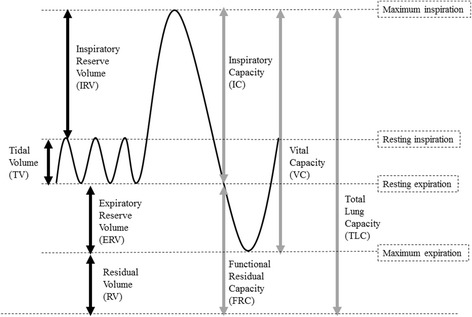
\includegraphics[scale=0.6]{imag/volumeslung.jpeg}
\caption{Medidas estándar de volumen pulmonar \cite{18}. }
\label{2}
\end{figure}
\FloatBarrier

%explicar proyecto


%Este proyecto abarca con la posibilidad de que un fisioterapeuta pueda realizar una prescripción y luego pueda revisar los resultados de un incentivo respiratorio.

%\subsubsection{Ejercicio de Fisioterapia para Paciente}

%complementar informacion

%A continuación se describen los tipos de ejercicios con sus características:

%\textbf{Patrón Diafragmático} \\
%Es un ejercicio que se encarga de lograr una capacidad residual funcional del paciente por medio de la inspiración nasal y espiración bucal. 


%\textbf{Inspiración Profunda}\\
%Es un ejercicio que se encarga de alcanzar la capacidad inspiratoria máxima (Volumen corriente VC + volumen de reserva inspiratorio VRI) mediante lo siguiente:
%\begin{itemize}
 %   \item Realizar una inspiración nasal lenta. 
  %  \item Realizar una apnea de 3 a 10 segundos. 
  %  \item Realizar una espiración lenta por la boca. 
%\end{itemize}

%\textbf{Inspiración fraccionada en el tiempo}\\
%La utilización de varias inspiraciones dentro del mismo ciclo ventilatorio, favorece la utilización de la capacidad inspiratoria en su plenitud con finalidad re-expansiva. Consiste en inspiraciones suaves y cortas por vía nasal e interrumpidas por cortos periodos de apnea (mínimo dos segundos cada uno) post inspiratoria programadas hasta en seis tiempos consecutivos, la espiración se da por la boca hasta el nivel de reposo inspiratorio o se extiende hasta el volumen medio de reserva inspiratoria.(4)
%El terapeuta determina en cuantas inspiraciones se llevará a cabo ya que puede ser inspiración fraccionada en 2 tiempo (realizar dos inspiraciones con los parámetros anteriores), en 3 tiempo 
%\begin{itemize}
 %   \item Inspiración nasal suave y corta
 %   \item Post inspiración realizar un periodo de apnea de mínimo dos segundos
 %   \item Se realizan hasta seis inspiraciones.
 %   \item Realizar una espiración suave por la boca
%\end{itemize}

%\textbf{Suspiros Inspiratorios}\\
%Este ejercicio se trata de una inspiración subdividida en inspiraciones cortas y sucesivas, sin apneas hasta que el paciente pueda contemplar la máxima capacidad inspiratoria




%\textbf{Espiración abreviada}\\
%Este ejercicio esta dado por 3 fases:
%\begin{itemize}
 %   \item Fase 1: Inspiración suave y profunda, espirando una pequeña cantidad de aire
  %  \item Fase 2: Vuelve a inspirar profundamente a partir del termino de la primera fase, espira nuevamente una pequeña cantidad de aire.
  %  \item Fase 3: vuelve a inspirar profundamente a partir del termino de la segunda fase, espirando completamente
%\end{itemize}



%\textbf{Ciclo Activo}\\
%Se encarga especialmente de repetir un ejercicio de patrón diafragmático o cualquiera de los ejercicios anteriores según el fisiofisioterapeuta lo determine para el paciente asignado.



\subsubsection{Capacidad vital} 

En espirometría es el volumen máximo que se puede inspirar y espirar en condiciones normales, se puede calcular teniendo en cuenta la siguiente ecuación \cite{50}.

\textbf{Para hombre:}

\begin{equation}
 CV (cm^3)= (27,63 – 0,112 * edad)* altura (cm)
\end{equation}


\textbf{Para mujer:}
    
\begin{equation}
   CV (cm^3)= (21,78 – 0,101 * edad) * altura (cm)
\end{equation}


Dentro de los parámetros espirómetricos también se encuentra definida la capacidad vital forzada CVF que es la cantidad máxima de aire exhalado forzadamente partiendo de una inhalación total; el pico de flujo espiratorio PEF como flujo instantáneo máximo de la maniobra CVF \cite{29}. El volumen espiratorio forzado en el primer segundo VEF1 se conoce como cantidad del aire exhalado abruptamente en el primer segundo después de una inhalación máxima. 



\subsubsection{Visualización de datos espirométricos}  %investigar

Los datos de inspirómetro o espirométricos se ven como gráficos llamados \textit{espirogramas} donde se muestran las medidas del volumen exhalado, el tiempo y las tasas de flujo de aire. Hay dos tipos de espirogramas estándar que se utiliza un fisioterapeuta respiratorio para evaluar cómo funcionan los pulmones, a continuación las medidas estándar que un fisioterapeuta evalúa durante la visualización de los datos: 

\begin{itemize}
    \item \textbf{Curva de volumen - tiempo}: Contiene los puntos de medición correspondientes a VEF1 = volumen espiratorio forzado en el primer segundo, FVC = capacidad vital forzada y EOTV = volumen al final de la espiración, como se puede ver en la figura \ref{3} de a continuación donde se observan los criterios de aceptabilidad (puntos máximos y mínimos ), los criterios de evaluación que utiliza un fisioterapeuta con la curva de comportamiento en rojo que se resalta, el eje horizontal para representar el tiempo en segundos y el eje vertical para representar el volumen:

        \begin{figure}[ht]
        \centering
        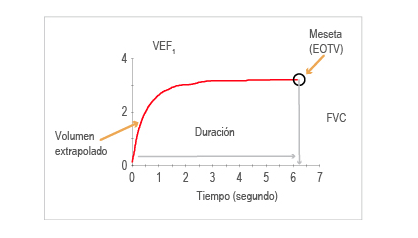
\includegraphics[scale=0.7]{imag/vvstiempo.png}
        \caption{Curva de volumen vs. tiempo \cite{36}. }
        \label{3}
        \end{figure}
        \FloatBarrier

    
    \item \textbf{Curva de flujo - volumen}: Muestra las tasas de flujo de aire en función del volumen exhalado. Esta curva como se muestra en la figura  \ref{4} a continuación,  contiene puntos correspondientes al PEF = pico espiratorio de flujo y al igual que la curva anterior se observan los criterios de aceptabilidad, criterios de evaluación del fisioterapeuta, el eje horizontal para representar el tiempo en segundos y el eje vertical para representar el flujo:
    
        \begin{figure}[ht]
        \centering
        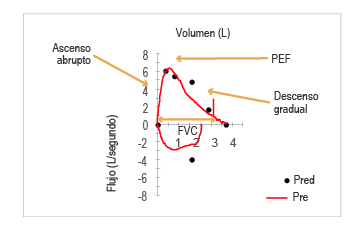
\includegraphics[scale=0.7]{imag/flujovs.png}
        \caption{Curva de flujo vs. volumen \cite{36}. }
        \label{4}
        \end{figure}
        \FloatBarrier
    
    
\end{itemize}



Para la visualización de los datos del proyecto se definió que la curva flujo - volumen se establece bajo un rango de variación de flujo respiratorio de  0 - 1200 centímetros cúbicos por segundo teniendo en cuenta que el fisioterapeuta respiratorio necesita conocer cuando el paciente ha logrado alcanzar 600, 900 y 1200 centímetros cúbicos por segundo definidos por el grupo de investigación en conjunto con los fisioterapeutas \cite{45}. El sistema web es capaz de representar en gráficas los datos de flujo que se extraen desde un inspirómetro con las medidas en centímetros cúbicos por segundo sin modificar su muestreo y después calcular la gráfica de volumen a partir de los datos de flujo.


\subsubsection{Prescripción}

El fisioterapeuta respiratorio puede realizar una prescripción con la asignación de las variables y valores correspondientes a cada uno de los datos definidos a continuación: 

\begin{itemize}
    \item \textbf{Frecuencia:} Cada cuantas horas se debe realizar un ejercicio, es determinada por el fisioterapeuta y se define por el número veces que realiza una sesión de fisioterapia, ejemplo: 3 series de 10 repeticiones, cada 8 horas, por una semana.
    \item \textbf{Duración:} Es el tiempo utilizado en la ejecución de una terapia.
    \item \textbf{Sesión:} Es la ejecución de un ejercicio en tiempo continuo en grupos de frecuencia.
    \item \textbf{Series:} Determinado por los momentos en una sola frecuencia.
    \item \textbf{Repeticiones:} Son las veces por serie de cada sesión
\end{itemize}
    

Se presenta las etapas de una prescripción en la figura \ref{5} a continuación:

\begin{figure}[htp]
\centering
\includegraphics[scale=0.6]{imag/ejemplopre.png}
\caption{Ejemplo de prescripción \cite{8}.}
\label{5}
\end{figure}
\FloatBarrier

Lo anterior, es un ejemplo de una prescripción específicamente cuando un paciente necesita alcanzar el 50-70\% de capacidad vital entre 3 series de 10 repeticiones con 1 minuto de descanso, en ese orden se evalúa por parte del fisioterapeuta.







%\subsubsection{Resultados de una Terapia Respiratoria}

%Cada paciente o participante de una terapia respiratoria debe tener realimentación de los resultados media





%-------------------------------------------------------------------------------------

%capítulo aparte

\clearpage

\section{Metodología de la Investigación}

La metodología considerada para el desarrollo del proyecto es TRIZ lo cual permite clasificar los atributos y características para definir los requerimientos del sistema inspirómetro, esta metodología se desarrolla en conjunto con el grupo de investigación de la Pontificia Universidad Javeriana Cali donde se integran áreas de fisioterapia, ingeniería de sistemas, ingeniería electrónica, diseño, ingeniería de software para desarrollar un sistema que permita realizar una terapia respiratoria y tenga realimentación visual para los usuarios, se plantea entonces los atributos del sistema en pasado, presente y futuro en nueve ventanas en la figura \ref{6} a continuación:

\begin{figure}[ht]
\centering
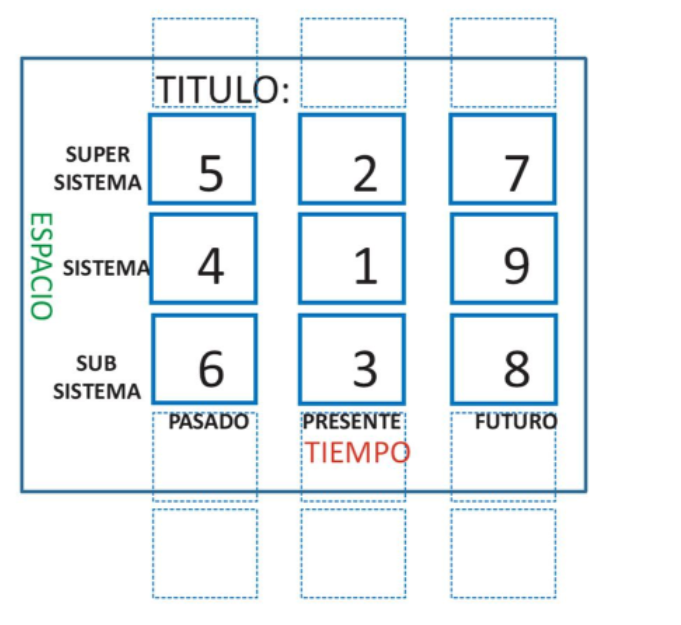
\includegraphics[scale=0.45]{imag/9ventanas.png}
\caption{Diagrama de nueve ventanas de metodología TRIZ \cite{37}. }
\label{6}
\end{figure}
\FloatBarrier


Para definir los requerimientos funcionales del sistema software, se analizaron cada una de las ventanas con el procedimiento indicado:
%fases de la metodología en diagrama %deio

\subsection{Sistema Presente} 

%\subsubsection{Ventana 1}
En la ventana 1 se analizaron los diferentes elementos de ayuda para la recuperación pulmonar de un paciente con sistemas actuales, se identifica que estos sistemas siempre van acompañados de una terapia denominada fisioterapia respiratoria, que como se explico anteriormente, es la encargada de definir que tipo de fisioterapia es la mejor para cada complicación respiratoria.

%\subsubsection{Ventana 2} 

En la ventana 2 se realiza el  análisis del super sistema, lo cual es en contexto donde se describen los elementos de ayuda para la recuperación de la capacidad pulmonar, en esta ventana se analizan las entidades o empresas que trabajan en la recuperación de la salud respiratoria, como también otros sectores relacionados con complicaciones respiratorias. En medicina, se utiliza respiración asistida en procesamientos quirúrgicos, donde se tienen en cuenta también técnicas respiratorias y fármacos para personas con enfermedades pulmonares. En industria, existen empresas que realizan el diseño y construcción de áreas limpias, manejo y control de ambientes hospitalarios y farmacéuticos. En lo social, esta directamente relacionado con el contagio de COVID por las personas que necesitan un tratamiento respiratorio asistido.

%\subsubsection{Ventana 3}

En la ventana 3 se realiza el  análisis del subsistema, donde se muestra de que están compuestos los diferentes elementos  investigados asociados a la recuperación de la capacidad pulmonar. Actualmente, se utilizan técnicas para la recuperación pulmonar de las personas, que se basan en una serie de instrucciones que el paciente debe seguir de acuerdo a la recomendación médica. Con un inspirómetro un paciente debe inhalar a través de la boquilla, lo que hace que la presión caiga dentro del dispositivo y, a su vez, hace que las bolas se eleven en cada uno de los tubos de flujo. Cada tubo está calibrado para que el desplazamiento completo de la pelota sea igual a un flujo específico, que se indica en la pared del tubo. El número de bolas y el nivel al que se elevan depende del nivel de flujo alcanzado \cite{38}. 

%https://patentimages.storage.googleapis.com/e3/b0/03/fefa9df55c113e/US20190134460A1.pdf

% investigar a nivel de software


En esta primera etapa y análisis de la metodologías utilizadas en sistemas actuales, se identifica que una terapia respiratoria no se realiza adecuadamente debido a la falta de adherencia hacia la actividad por parte del paciente, además no existe un seguimiento con datos registrados que el fisioterapeuta pueda evaluar, no hay un registro tampoco de un histórico de la evolución del paciente quien requiere principalmente indicaciones previas del fisioterapeuta respiratorio.

\subsection{Sistema Pasado}

%\subsubsection{Ventana 4}

En la ventana 4 se abarcar el tema de la rehabilitación pulmonar abarca desde los comienzos del arte médico, con ello, las principales estrategias utilizadas para disminuir el impacto de la enfermedad pulmonar crónica, las terapias recomendadas eran el reposo, evitar situaciones de esfuerzo físico o por el contrario entrenamientos físico con miras a rehabilitar los pacientes con el máximo posible de alcance de su sistema pulmonar y después de ello, también se desarrollaron técnicas aplicando los principios científicos entre los cuales vemos el entrenamiento muscular y oxígeno-terapia crónica domiciliaria.

%\subsubsection{Ventana 5}

En la ventana 5 se considera que en el pasado no se tenía la conciencia de prevenir ciertos tipos de enfermedades como las respiratorias, de hecho no existían grandes compañías dedicadas al cuidado o rehabilitación de la capacidad pulmonar como las hay hoy en día. Solo existían esfuerzos e investigaciones individuales cuyas conclusiones permitieron que se desarrolle la industria que actualmente existe.

%\subsubsection{Ventana 6}

En la ventana 6 se menciona que en el pasado no existía una gran preocupación sobre enfermedades respiratorias y en general como las hay hoy en día, no había dispositivos que ayudaran a la recuperación pulmonar de las personas, salvo ejercicios de respiración que aún se usan en la fisioterapia respiratoria. 




\subsection{Sistema Futuro} 

%\subsubsection{Ventana 7}

En la ventana 7 se analiza en cuanto al futuro donde se entra al plano imaginario, en este caso el contexto en el que se encontraran los elementos de recuperación pulmonar. En medicina uno de los aspectos a mejorar es la de la reducción de tiempos de convalecencia en los hospitales porque minimiza costos tanto al hospital como al paciente además abre espacio para pacientes con otras patologías y una de las tendencias para lograr esto es la fisioterapia domiciliaria, que el paciente realice su terapia desde la comodidad de su casa y no tenga de desplazarse hasta el hospital. Desde lo social y ambiental, estos temas van de la mano debido a que en algunos países no se está trabajando lo suficiente en lo ambiental lo cual significa un aumento en la contaminación del aire que respiran las personas sobre todo en las grandes ciudades, lo cual también aumentaría la probabilidad de adquirir algunas afección respiratoria y sin tratamiento podría aumentar la tasa de mortalidad por estas causas. 

%\subsubsection{Ventana 8}

En la ventana 8 el sistema ideado deberá usar algoritmos de programación para el envío y recepción de datos además de generar un reporte de datos de lo realizado por el paciente en el cual el profesional de la salud analizará el rendimiento del paciente.

%\subsubsection{Ventana 9}

En la ventana 9 el software del inspirómetro deberá ser capaz de ejecutarse en un sistema operativo común, con el fin de tener mayores posibilidades de uso.  Además deberá tener una interfaz gráfica intuitiva para que tanto el paciente como el fisioterapeuta puedan usarlo de manera fácil y adecuada. Dicha interfaz deberá permitir modificar los límites de trabajo por parte del fisioterapeuta con el fin de adaptar la terapia a los pacientes con mayores dificultades respiratorias. 


Con lo anterior y dadas las características y atributos de los sistemas en pasado y presente, el sistema futuro, debe permitir que el paciente se pueda concentrar en su terapia y hacerla conscientemente, permitir adquirir datos, codificar, presentar y almacenar la información de desempeño de la terapia tanto al paciente como al fisioterapeuta mediante una conexión remota, debe permitir la administración de usuarios, una plataforma con operaciones intuitivas para la programación de ejercicios para cada sesión y que permita la prescripción remoto de los mismos.

%-------------------------------------------------------------------------------------
\newpage
\section{Proceso de Ingeniería de Software  } %desarrollo del software (perfil del terapueta)

%incluir diagrama de casos de uso con explicación

%que se obtuvo en cada una de las fases, el proyecto grande utilizo las nueve ventanas despues de ello surgio la arquitectura de referencia, seccion global, proyecto grande, contar resultados resumidos, requesitos genericos y luego el desarrollo de software, 

Bajo los atributos identificados con la metodología TRIZ se desarrollan a continuación los requerimientos funcionales y no funcionales del sistema software propuesto.


\subsection{Definición de Requerimientos del Sistema}

En esta sección se detallan los procesos realizados para obtener los requerimientos del sistema, la estructura y documentación de los requerimientos, validación y priorización de estos.

\subsubsection{Diagrama de contexto} %explicar 

Contiene todos los posibles escenarios, personas, documentación que interactúan, aportan datos e información para el sistema software del inspirómetro, cada zona representada con colores distintos que muestran la relación entre ellas y el contexto de la información que se aporta al sistema, en este caso, las zonas azules son las que se identifican para el sistema software de fisioterapia respiratoria, también se tiene en cuentan las zonas grises para representar una posible regulación de tratamiento de datos que son por las partes interesadas, lo anterior, se observa en la figura \ref{7} a continuación:

\begin{figure}[ht]
\centering
\includegraphics[scale=0.40]{imag/C4-Diagram contexto.drawio (1).png}
\caption{Diagrama de contexto de sistema software de inspirómetro. }
\label{7}
\end{figure}
\FloatBarrier

\newpage

\subsubsection{Diagrama de casos de uso} %explicar 

Se identificaron las posibles relaciones mediante un diagrama de casos de usos que permitió exponer el comportamiento deseado del sistema. En la figura \ref{8} se muestra la inclusión de los procesos que incorpora explícitamente el comportamiento de un caso de uso, como también se muestra la extensión como sub-funciones de un caso de usos.


\begin{figure}[ht]
\centering
\includegraphics[scale=0.45]{imag/C4-Caso Usos.png}
\caption{Diagrama de casos de uso para aplicación web }
\label{8}
\end{figure}
\FloatBarrier

El diagrama permite definir las acciones especificas y principales que debe realizar el fisioterapeuta respiratorio, mostrado de color azul las funciones de gestionar pacientes, prescribir, consultar el estado de pacientes y realizar el diagnóstico a partir de los datos que han sido trasmitidos al sistema web, con la relación de \textit{include} y  \textit{extend} para mostrar las sub-funciones de cada una de ellas. Por otro lado, están las funciones del paciente en gris que el sistema no desarrolla directamente pero tiene en cuenta para definir los servicios que se van a desarrollar para la comunicación de datos.


\subsubsection{Diagrama de flujo general de la aplicación web} %explicar 

Como parte de las tareas principales que debe realizar el fisioterapeuta es la de asignar una prescripción y valorar el paciente dada la gráfica de comportamiento del flujo respiratorio por usuario, los datos obtenidos durante una fisioterapia son procesados desde un dispositivo inspirómetro y son enviados hacia la aplicación web para ser visualizadas. Se presenta a continuación el diagrama de flujo la figura \ref{9} cuando el fisioterapeuta ingresa a la aplicación web: 


\begin{figure}[ht]
\centering
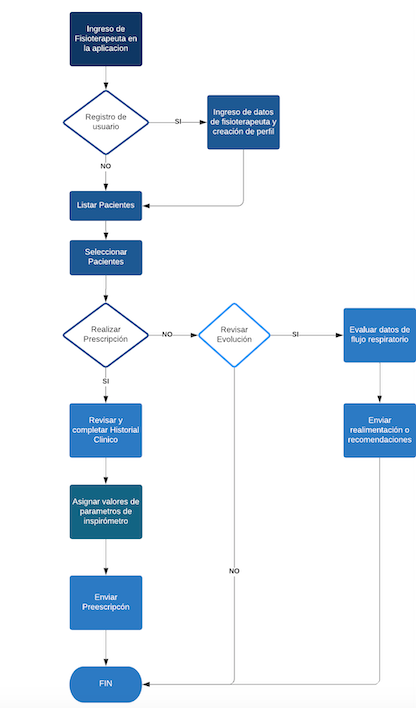
\includegraphics[scale=0.622]{imag/DiagramaFlujo.png}
\caption{Diagrama de flujo general para sistema web }
\label{9}
\end{figure}
\FloatBarrier


Con el diagrama de flujo se valida la acción desde el paso inicial hasta final para dar un primer acercamiento detallado sobre como debe navegar un fisioterapeuta en el sistema web para que pueda completar un envío de prescripción para una fisioterapia respiratoria. Se representa desde el inicio el ingreso del fisioterapeuta a la aplicación
y como deber responder la aplicación según la acción que va a realizar de las disponibles, ya sea un registro de usuario o ver los pacientes que tiene registrados, mas adelante se representa en modelo de decisión, la etapa de realizar prescripción y revisar evolución, seguido de los procesos que corresponden a cada decisión con un azul diferente dado a que hacen parte de la etapa en la que se encuentra el usuario resultando en verde tenue la etapa mas importante que es la de asignar los valores de parámetros de inspirómetro. 


\subsubsection{Técnicas de obtención de requerimientos}

\begin{enumerate}
    \item \textbf{Reuniones grupales:} Inicialmente ser realizan reuniones grupales con los principales actores del sistema, tanto los posibles usuarios como fisioterapeuta respiratorio como los desarrolladores del sistema de las diferentes áreas, software, electrónica y diseño.
    \item \textbf{Encuestas:} 
        \begin{enumerate}
            \item Encuesta dirigida a fisioterapeutas tanto externos como internos del proyecto, con el propósito de identificar atributos comunes con los mencionados en el grupo de investigación, para lograr el objetivo, se realizaron preguntas orientadas a las terapias respiratorias, los datos que se evalúan actualmente y las metodologías utilizadas.
            \item Encuesta dirigida a los pacientes con el fin de conocer la experiencia de los pacientes que han realizado terapia respiratoria con el inspirómetro incentivo en cuanto a la terapia y el acompañamiento con el terapeuta.
        \end{enumerate}
        
    \item \textbf{Prototipado:} 
    
        \begin{enumerate}
            \item Se definieron vistas e interacción de usuario, en este caso, como el fisioterapeuta deberá desenvolver en la aplicación web, como el registro de pacientes, realización de la prescripción y la visualización de resultados para el diagnóstico.
        \end{enumerate}
    
    
\end{enumerate}




\subsubsection{Definición de requerimientos funcionales}

%Modulo Fisioterapeuta============================================ 

 % FUNCIÓN EVALUAR
\begin{enumerate}[start=1,label={\bfseries RF0\arabic*.}]

    \item El sistema debe tener una funcionalidad para el fisioterapeuta respiratorio que le permita evaluar el estado de un paciente. 
    %para una sesión realizada por un paciente 
        \label{RF01}
            \begin{enumerate}[label*=\arabic*.]
                %datos específicos evalúa el fisio
                \item Permitir realizar un diagnóstico y posteriormente recetar la terapia correspondiente por paciente, si es necesario.
                
                \item Permitir la visualización de datos registrados como flujo respiratorio por cada sesión por medio de gráficas de desempeño.
                
                \item Permitir revisar la evolución del paciente dados los datos de flujo respiratorio de cada una de las terapias por sesión.
        
            \end{enumerate}

    %EJERCICIOS     --como quedan descritos? animaciones, textos ?
    \item El sistema debe tener una funcionalidad para al fisioterapeuta que le permita programar  una prescripción por cada sesión en el sistema web.
        
        \label{RF02}
            \begin{enumerate}[label*=\arabic*.]
            
                \item Se debe permitir cargar una prescripción con valores numéricos enteros. %completar si son descritos, texto o con animaciones
                 
                \item Se debe permitir el almacenamiento de prescripciones con valores asignados por paciente. %completar
                
                \item Se debe permitir modificar, cargar o eliminar prescripciones.
                
                \item Se debe permitir establecer parámetros de prescripciones por conexión remota.
                
     
                
            \end{enumerate}
            
    %ORIENTAR
    \item  El sistema debe tener una funcionalidad para al fisioterapeuta que le permita orientarse en el manejo de las prescripciones.
    
    \label{RF03}
            \begin{enumerate}[label*=\arabic*.]
                %Posible requerimiento
                \item Se debe incluir una función de usuario que permita ver una secuencia de uso de la aplicación correctamente. 
            \end{enumerate}
            
    
    %PACIENTES
    \item  El sistema debe tener una funcionalidad para al fisioterapeuta que le permita la gestión de los parámetros de cada sesión por medio de los perfiles de cada paciente, parámetros tales como  el rango de medición de flujo inspirado, volumen, frecuencia respiratoria y saturación de oxígeno por cada paciente. %preguntar       
    \label{RF04}
            \begin{enumerate}[label*=\arabic*.]
                \item La funcionalidad de gestión de parámetros que le permita al fisioterapeuta establecer rangos en volumen, frecuencia y saturación de oxígeno por medio de teleconsulta. %videollamada?
                
                \item La funcionalidad para al fisioterapeuta debe permitir establecer parámetros de flujo inspirado y asignar los ejercicios correspondientes por paciente
                
                
            \end{enumerate}
            
    %DIAGNOSTICO
    \item El sistema debe tener una funcionalidad para al fisioterapeuta que le permita realizar un diagnóstico dados los datos de flujo respiratorio del paciente visualizados en gráficas de comportamiento.
    

    
    
    %ALMACENAR DATOS
    \item El sistema debe tener una funcionalidad para al fisioterapeuta que le permita guardar los cambios realizados en la plataforma como las modificaciones de las prescripciones en cada una de las sesiones de terapia.
    
    
    
            
%Modulo Paciente===================================================================

 %ORIENTAR
   % \item El sistema debe tener una funcionalidad que permita orientar al fisioterapeuta  para la realización de un ejercicio de una terapia respiratoria. 
    %\label{RF08}
     %       \begin{enumerate}[label*=\arabic*.]
            
      %          \item La funcionalidad de orientar al paciente debe incluir una demostración con los pasos o secuencia a seguir sobre como manejar la aplicación, como usar el inspirómetro electrónico y como realizar el ejercicio prescrito.
                
       %         \item La funcionalidad de orientar al paciente de manera sensitiva debe permitir generar una secuencia en la terapia por cada sesión establecida al paciente, los ejercicios permitirán el estimulo que el paciente  necesita para su recuperación. %que serían las cualidades de la orientación
                
        %        \item La funcionalidad de orientar al paciente debe contar con una guía de usuario que debe incluir una demostración con los pasos o secuencia a seguir sobre como manejar la aplicación.
                
         %       \item La funcionalidad de orientar al paciente debe contar con un realimentación después de una sesión realizada que permita dar a conocer resultados y consejos de avance en terapia para una próxima sesión, esta funcionalidad se dará con la intervención del terapeuta al finalizar cada sesión.
    
          %      \item La funcionalidad de orientar al paciente debe mostrar datos de evolución que permitan conocer el estado en que se encuentra el paciente para completar una terapia respiratoria.
                
           %     \item La funcionalidad de orientar al paciente debe contar con una guía sobre como usar el inspirómetro electrónico y como realizar el ejercicio prescrito, resaltando también los limites de seguridad del sistema.
        %    \end{enumerate}
            
            
        %enviar realimentacion por otros medios no solo visual

%Modulo de  Administración============================================    

 
    \item El sistema debe contar con una estructura de gestión de usuarios.
    %Grupos de pacientes  
    \item El sistema debe permitir a los fisioterapeutas administrar grupos de pacientes para asignar las respectivas prescripciones.
    \label{RF10}
        \begin{enumerate}[label*=\arabic*.]
            \item Permitir a los fisioterapeutas la creación y administración de grupos de pacientes, los cuales van a tener en su plataforma registrados con los datos demográficos de cada paciente.
            
        \end{enumerate}
        
  
            

         
    
%Modulo sistema central de procesamiento===========================================
 
    
    %Adquirir datos
    
    \item El sistema debe permitir adquirir, almacenar y presentar al fisioterapeuta los datos de flujo respiratorio  como desempeño del paciente estimados en una sesión por conexión remota.
    
     \label{RF12}
            \begin{enumerate}[label*=\arabic*.]
                
                \item El sistema debe tener una funcionalidad de toma de datos de flujo respiratorio del paciente que permita agrupar la captura de datos en un historial.
                
                \item El sistema debe tener una funcionalidad de toma de datos del paciente que permita hacer el registro de datos de flujo respiratorio mediante los estímulos capturados uno a uno desde el inspirómetro con un método cuantitativo de grabación de datos.  %evaluar
                
                \item El sistema debe tener una funcionalidad de codificar la variable física medida con el inspirómetro a partir de los datos derivados del flujo respiratorio y presentarlos graficados en la aplicación web. %Codificar la información de la variable física medida. (estructura de datos)
            
            \end{enumerate}
        

      
    %Trasmisión de datos=================================
    
    
    \item El sistema debe contar con una API para permitir la trasmisión de datos.
    
   
    
    %Almacenamiento de datos
    
   
    \item El sistema debe permitir la funcionalidad de registro de datos del paciente para garantizar el auto-guardado por cada ejercicio realizado.
    
    
  
    
    
    %Gamificación
    \item El sistema web debe permitir integrar un módulo de gamificación para acoplarse con un sistema móvil para la presentación de  prescripciones y  de datos de comportamiento de  flujo respiratorio.
    
     
    
    %%Juego
    %\item El sistema debe permitir mantener un flujo  respiratorio constante indicado en los ejercicios prescritos por el fisioterapeuta.
    %porque eso le va a permitir que el flujo de aire llegue a los alveolos y realice el íntercambio, La parte de ser constante y laminar hace que la bolita o lo que se mira en el incentivo, Este quieta en un solo lugar, Sin subir o bajar,Entonces esa bolita quieta y a la altura  me permite saber que si lo esta haciendo bien, Si, pues dependiendo del volumen a donde el profesional le indique a la persona llegar. Ya que el dispositivo tiene aun lado marcado como en rayitas los niveles de volumen que se esta alcanzando
    %\label{RF21}
     %       \begin{enumerate}[label*=\arabic*.]
            
      %          \item El sistema debe permitir la funcionalidad de mantener un flujo y volumen constante en cada sesión para registrar los niveles de volumen y frecuencia respiratoria 
       %     \end{enumerate}
    
        

%https://www.gloomaps.com/3zr2f3aYfo

\end{enumerate}


\subsubsection{Definición de requerimientos de calidad}

\begin{enumerate}[start=1,label={\bfseries RNF\arabic*.}]


%\item  El sistema debe ser exigente en tecnología para que pueda ser usado por cualquier paciente con un sistema tecnológico de comunicación. %Android

%\item El sistema debe estar en la capacidad de funcionar en modo offline, es decir soporte sin conexión, cuando las condiciones de conexión con el servidor sean adversas, asegurando que la información no se pierda a causa de estos imprevistos

\item El sistema debe permitir que cualquier usuario que no conozca a profundidad el funcionamiento de las TIC tenga un buen desempeño con el manejo de la herramienta.

%\item El sistema debe asegurar una disponibilidad del 99.0 \%

%\item El sistema debe ser desarrollado bajo los principios de diseño SOLID

%\item El sistema debe tener un tiempo TTI menor o igual a 5 segundos

 \item El sistema debe cumplir con parámetros ACID para el relacionamiento con bases de datos.
 
%\item El sistema debe contar con las características necesarias para hacer un deploy sencillo

%\item El sistema debe contar con una función de backup y de recuperación ante fallos
\item El sistema debe soportar concurrencia de múltiples usuarios.
%\item El sistema debe contar con los protocolos necesarios para asegurar un funcionamiento seguro a través de Internet, es decir, que la información enviada y recibida este protegida contra ataques de robo información y suplantación de identidad. 
%\item El sistema no debería ser invasivo.
        
\item El sistema debe favorecer la adherencia al tratamiento de fisioterapia.

\end{enumerate}




\subsubsection{Definición de requerimientos tipo restricción}

\begin{enumerate}[start=1,label={\bfseries RTR\arabic*.}]

\item Poner el mínimo número de comandos de operación para el fisioterapeuta.


\end{enumerate}


\subsubsection{Especificación y priorización de requerimientos}
%-------------------------------------------------------------------------------------

A continuación se presenta los requerimientos funcionales con su respectiva especificación y validación dependiendo del la prioridad: alta, media o baja, respectivamente.


\begin{center}
\begin{tabular}{|c|c|p{4cm}|p{4cm}|}
            \hline
            \rowcolor{red} \multicolumn{4}{|c|}{\textbf{Prioridad:} Alta}  \\
            \hline
            \multicolumn{2}{|l}{\textbf{Nro.Requisito: }RF.01} & \multicolumn{1}{|l}{\textbf{Versión: 1.1}} & \multicolumn{1}{|l|}{\textbf{Estado: Aprobado}} \\
            \multicolumn{4}{|p{13cm}|}{\textbf{Caso de uso Nro: }}  \\
            \hline
            \multicolumn{4}{|p{13cm}|}{\textbf{Descripción: } El sistema debe tener una funcionalidad para el terapeuta respiratorio que le permita evaluar una sesión realizada por un paciente } \\
            \multicolumn{4}{|p{13cm}|}{\textbf{Justificación: } El fisioterapeuta solicita que la aplicación web le permita ver los datos del paciente y conocer la evolución del mismo.} \\ 
            \multicolumn{4}{|p{13cm}|}{\textbf{Origen: }Fisioterapeuta}  \\
            \multicolumn{4}{|p{13cm}|}{\textbf{Criterio de verificación: } El sistema web permite visualizar los datos registrados de una prescripción y conocer la evolución del paciente.  } \\
            \hline
            \multicolumn{4}{|p{13cm}|}{\textbf{Prerequisitos: } Todos los requisitos de prioridad alta. }\\
            \hline \multicolumn{4}{|p{12cm}|}{\textbf{Dependencias: }
                \begin{itemize}
                \item RF01.1
                \item RF01.2
                \item RF01.3
                \end{itemize}}  \\
            \multicolumn{4}{|p{12cm}|}{\textbf{Conflictos: }}  \\
            \hline
            \multicolumn{4}{|p{12cm}|}{\textbf{Documentos de soporte: }}  \\
            \hline
            \multicolumn{4}{|p{12cm}|}{\textbf{Historial del Requerimiento: }}  \\
            \multicolumn{4}{|p{12cm}|}{\textbf{Creación : }09/10/2021}  \\
            \multicolumn{4}{|p{12cm}|}{\textbf{Modificación: }}  \\
             \textbf{Versión} & \textbf{Fecha} & \multicolumn{2}{p{8cm}|}{\textbf{Cambio realizado:}} \\
            \hline
               1.1    &20/10/2021 &   \multicolumn{2}{p{8cm}|}{Se desarrolla prototipado para esta funcionalidad y se modifica los requisitos RF01.2 y RF01.3 en cuanto a visualizar los datos como flujo respiratorio y se crea el requisito RF01.1}
              \\
            \hline
        \end{tabular}

        
        \medskip
        
        
        %%%%%%%%%%%%%%%%%%%%%%%%%%%%%%%%%%%%%2
        
        
        \begin{tabular}{|c|c|p{4cm}|p{4cm}|}
            \hline
            \rowcolor{red} \multicolumn{4}{|c|}{\textbf{Prioridad:} Alta}  \\
            \hline
            \multicolumn{2}{|l}{\textbf{Nro.Requisito: }RF.02} & \multicolumn{1}{|l}{\textbf{Versión: 1.1}} & \multicolumn{1}{|l|}{\textbf{Estado: Aprobado}} \\
            \multicolumn{4}{|p{13cm}|}{\textbf{Caso de uso Nro: }}  \\
            \hline
            \multicolumn{4}{|p{13cm}|}{\textbf{Descripción: } El sistema debe tener una funcionalidad para el terapeuta respiratorio que le permita programar una prescripción por cada sesión en el sistema web } \\
            \multicolumn{4}{|p{13cm}|}{\textbf{Justificación: } El fisioterapeuta solicita que la aplicación web le permita programar una prescripción general por paciente.} \\ 
            \multicolumn{4}{|p{13cm}|}{\textbf{Origen: }Fisioterapeuta}  \\
            \multicolumn{4}{|p{13cm}|}{\textbf{Criterio de verificación: } El sistema web permite visualizar los datos registrados de una prescripción y conocer la evolución del paciente.  } \\
            \hline
            \multicolumn{4}{|p{13cm}|}{\textbf{Prerequisitos: } Todos los requisitos de prioridad alta. }\\
            \hline \multicolumn{4}{|p{12cm}|}{\textbf{Dependencias: }
                \begin{itemize}
                \item RF02.1
                \item RF02.2
                \item RF02.3
                \item RF02.4
                \end{itemize}}  \\
            \multicolumn{4}{|p{12cm}|}{\textbf{Conflictos: }}  \\
            \hline
            \multicolumn{4}{|p{12cm}|}{\textbf{Documentos de soporte: }}  \\
            \hline
            \multicolumn{4}{|p{12cm}|}{\textbf{Historial del Requerimiento: }}  \\
            \multicolumn{4}{|p{12cm}|}{\textbf{Creación : }09/10/2021}  \\
            \multicolumn{4}{|p{12cm}|}{\textbf{Modificación: }}  \\
             \textbf{Versión} & \textbf{Fecha} & \multicolumn{2}{p{8cm}|}{\textbf{Cambio realizado:}} \\
            \hline
               1.1    &20/10/2021 &   \multicolumn{2}{p{8cm}|}{Se desarrolla prototipado para esta funcionalidad y se modifica los requisitos RF02.1 y RF02.2 en cuanto a realizar una prescripción con campos para valores numéricos}
              \\
            \hline
        \end{tabular}

        
   %     \medskip
        
        
        
        
        
        
        %%%%%%%%%%%%%%%%%%%%%%%%%%%%%%%%%%%%
        
         \begin{tabular}{|c|c|p{4cm}|p{4cm}|}
            \hline
            \rowcolor{orange} \multicolumn{4}{|c|}{\textbf{Prioridad:} Media}  \\
            \hline
            \multicolumn{2}{|l}{\textbf{Nro.Requisito: }RF.03} & \multicolumn{1}{l|}{\textbf{Versión: }} & \multicolumn{1}{|l|}{\textbf{Estado: Aprobado}} \\
            \multicolumn{4}{|p{12cm}|}{\textbf{Caso de uso Nro: }}  \\
            \hline
            \multicolumn{4}{|p{13cm}|}{\textbf{Descripción: } El sistema debe tener una funcionalidad para al fisioterapeuta que le permita orientarse en el manejo de las prescripciones}  \\
            \multicolumn{4}{|p{13cm}|}{\textbf{Justificación: }Se sugiere al fisioterapeuta conocer la secuencia de pantallas de la interfaz web y como se esperan los datos}  \\
            \multicolumn{4}{|p{12cm}|}{\textbf{Origen: }Ingeniero de requisitos}  \\
            \multicolumn{4}{|p{13cm}|}{\textbf{Criterio de verificación: }}  \\
            \hline
            \multicolumn{4}{|p{13cm}|}{\textbf{Prerequisitos: }}  \\
            \hline
            \multicolumn{4}{|p{12cm}|}{\textbf{Dependencias: }
                \begin{itemize}
                \item RF03.1
                \end{itemize}}  \\
            \multicolumn{4}{|p{12cm}|}{\textbf{Conflictos: }}  \\
            \hline
            \multicolumn{4}{|p{12cm}|}{\textbf{Documentos de soporte: }}  \\
            \hline
            \multicolumn{4}{|p{12cm}|}{\textbf{Historial del Requerimiento: }}  \\
            \multicolumn{4}{|p{12cm}|}{\textbf{Creación : }20/09/2021}  \\
            \multicolumn{4}{|p{12cm}|}{\textbf{Modificación: }}  \\
             \textbf{Versión} & \textbf{Fecha} & \multicolumn{2}{p{8cm}|}{\textbf{Cambio realizado:}} \\
            \hline
               1.1    &31/10/2021 &   \multicolumn{2}{p{8cm}|}{se desarrolla prototipado para esta funcionalidad y se modifica el requisito RF03.1 en cuanto a orientar al fisioterapeuta}
              \\
            \hline
        \end{tabular}
        
        
        \begin{tabular}{|c|c|p{4cm}|p{4cm}|}
            \hline
            \rowcolor{yellow} \multicolumn{4}{|c|}{\textbf{Prioridad:} Baja}  \\
            \hline
            \multicolumn{2}{|l}{\textbf{Nro.Requisito: }RF.04} & \multicolumn{1}{l|}{\textbf{Versión: 1.1 }} & \multicolumn{1}{|l|}{\textbf{Estado: Aprobado}}  \\
            \multicolumn{4}{|p{12cm}|}{\textbf{Caso de uso Nro: }}  \\
            \hline
            \multicolumn{4}{|p{13cm}|}{\textbf{Descripción: }El sistema debe tener una funcionalidad para al fisioterapeuta que le permita la gestión de los parámetros de cada sesión por medio de los perfiles de cada paciente, parámetros tales como el rango de medición de flujo inspirado, volumen, frecuencia respiratoria por cada paciente.}  \\
            \multicolumn{4}{|p{13cm}|}{\textbf{Justificación: }El Fisioterapeuta solicita que la aplicación web le permita la gestión de parámetros para realizar una prescripción}  \\
            \multicolumn{4}{|p{12cm}|}{\textbf{Origen: }Fisioterapeuta}  \\
            \multicolumn{4}{|p{13cm}|}{\textbf{Criterio de verificación: }}  \\
            \hline
            \multicolumn{4}{|p{13cm}|}{\textbf{Prerequisitos: }}  \\
            \hline \multicolumn{4}{|p{12cm}|}{\textbf{Dependencias: }
                \begin{itemize}
                \item RF04.1
                \item RF04.2
                \end{itemize}}  \\
            \multicolumn{4}{|p{12cm}|}{\textbf{Conflictos: }}  \\
            \hline
            \multicolumn{4}{|p{12cm}|}{\textbf{Documentos de soporte: }}  \\
            \hline
            \multicolumn{4}{|p{12cm}|}{\textbf{Historial del Requerimiento: }}  \\
            \multicolumn{4}{|p{12cm}|}{\textbf{Creación : }20/09/2021}  \\
            \multicolumn{4}{|p{12cm}|}{\textbf{Modificación: }}  \\
             \textbf{Versión} & \textbf{Fecha} & \multicolumn{2}{p{8cm}|}{\textbf{Cambio realizado:}} \\
            \hline
               1.1    &31/10/2021 &   \multicolumn{2}{p{8cm}|}{Se desarrolla prototipado para esta funcionalidad y se modifica los requisitos RF04.1 en cuanto a establecer parámetros generales de prescripción y se crea el requisito RF04.2}
              \\
            \hline
        \end{tabular}
        
        

\begin{tabular}{|c|c|p{4cm}|p{4cm}|}
            \hline
            \rowcolor{red} \multicolumn{4}{|c|}{\textbf{Prioridad:} Alta}  \\
            \hline
            \multicolumn{2}{|l}{\textbf{Nro.Requisito: }RF.05} & \multicolumn{1}{|l}{\textbf{Versión: 1.1}} & \multicolumn{1}{|l|}{\textbf{Estado: Aprobado}} \\
            \multicolumn{4}{|p{13cm}|}{\textbf{Caso de uso Nro: }}  \\
            \hline
            \multicolumn{4}{|p{13cm}|}{\textbf{Descripción: } El sistema debe tener una funcionalidad para al fisioterapeuta que le permita realizar un diagnostico dados los datos de flujo respiratorio del paciente visualizados en gráficas de comportamiento. } \\
            \multicolumn{4}{|p{13cm}|}{\textbf{Justificación: } El fisioterapeuta solicita que la aplicación web le permita ver el comportamiento de flujo respiratorio del paciente y conocer la evolución del mismo.} \\ 
            \multicolumn{4}{|p{13cm}|}{\textbf{Origen: }Fisioterapeuta}  \\
            \multicolumn{4}{|p{13cm}|}{\textbf{Criterio de verificación: } El sistema web permite visualizar los datos de flujo respiratorio del paciente.  } \\
            \hline
            \multicolumn{4}{|p{13cm}|}{\textbf{Prerequisitos: } Todos los requisitos de prioridad alta. }\\
            \hline \multicolumn{4}{|p{12cm}|}{\textbf{Dependencias: }
                }  \\
            \multicolumn{4}{|p{12cm}|}{\textbf{Conflictos: }}  \\
            \hline
            \multicolumn{4}{|p{12cm}|}{\textbf{Documentos de soporte: }}  \\
            \hline
            \multicolumn{4}{|p{12cm}|}{\textbf{Historial del Requerimiento: }}  \\
            \multicolumn{4}{|p{12cm}|}{\textbf{Creación : }09/10/2021}  \\
            \multicolumn{4}{|p{12cm}|}{\textbf{Modificación: }}  \\
             \textbf{Versión} & \textbf{Fecha} & \multicolumn{2}{p{8cm}|}{\textbf{Cambio realizado:}} \\
            \hline
               1.1    &20/10/2021 &   \multicolumn{2}{p{8cm}|}{Se desarrolla prototipado para esta funcionalidad y  se modifica los requisitos RF05 en cuanto a visualizar los datos como comportamiento de flujo respiratorio}
              \\
            \hline
\end{tabular}

        
        %\medskip
        
        
        
        
        \begin{tabular}{|c|c|p{4cm}|p{4cm}|}
            \hline
            \rowcolor{yellow} \multicolumn{4}{|c|}{\textbf{Prioridad:} Baja}  \\
            \hline
            \multicolumn{2}{|l}{\textbf{Nro.Requisito: }RF.06} & \multicolumn{1}{l|}{\textbf{Versión: }} & \multicolumn{1}{|l|}{\textbf{Estado: Aprobado}}  \\
            \multicolumn{4}{|p{12cm}|}{\textbf{Caso de uso Nro: }}  \\
            \hline
            \multicolumn{4}{|p{13cm}|}{\textbf{Descripción: }El sistema debe tener una funcionalidad de envío de vídeos para brindar realimentaciones de manera cualitativa e instrucciones necesarias para la terapia}  \\
            \multicolumn{4}{|p{13cm}|}{\textbf{Justificación: }El Fisioterapeuta solicita que la aplicación web tenga funcionalidad de envió de vídeos}  \\
            \multicolumn{4}{|p{12cm}|}{\textbf{Origen: }Fisioterapeuta}  \\
            \multicolumn{4}{|p{13cm}|}{\textbf{Criterio de verificación: }}  \\
            \hline
            \multicolumn{4}{|p{13cm}|}{\textbf{Prerequisitos: }}  \\
            \hline \multicolumn{4}{|p{12cm}|}{\textbf{Dependencias: }
               }  \\
            \multicolumn{4}{|p{12cm}|}{\textbf{Conflictos: }}  \\
            \hline
            \multicolumn{4}{|p{12cm}|}{\textbf{Documentos de soporte: }}  \\
            \hline
            \multicolumn{4}{|p{12cm}|}{\textbf{Historial del Requerimiento: }}  \\
            \multicolumn{4}{|p{12cm}|}{\textbf{Creación : }20/09/2021}  \\
            \multicolumn{4}{|p{12cm}|}{\textbf{Modificación: }}  \\
             \textbf{Versión} & \textbf{Fecha} & \multicolumn{2}{p{8cm}|}{\textbf{Cambio realizado:}} \\
            \hline
                    & &   \multicolumn{2}{p{8cm}|}{}
              \\
            \hline
        \end{tabular}
        
        
        
        
        
        
        
\begin{tabular}{|c|c|p{4cm}|p{4cm}|}
            \hline
            \rowcolor{red} \multicolumn{4}{|c|}{\textbf{Prioridad:} Alta}  \\
            \hline
            \multicolumn{2}{|l}{\textbf{Nro.Requisito: }RF.07} & \multicolumn{1}{|l}{\textbf{Versión:}} & \multicolumn{1}{|l|}{\textbf{Estado: Aprobado}} \\
            \multicolumn{4}{|p{13cm}|}{\textbf{Caso de uso Nro: }}  \\
            \hline
            \multicolumn{4}{|p{13cm}|}{\textbf{Descripción: } El sistema debe tener una funcionalidad para al fisioterapeuta que le permita guardar los cambios realizados en la plataforma como las modificaciones de las prescripciones en cada una de las sesiones de terapia. } \\
            \multicolumn{4}{|p{13cm}|}{\textbf{Justificación: } El fisioterapeuta solicita que la aplicación web le permita guardar las modificaciones necesarias en una prescripción } \\ 
            \multicolumn{4}{|p{13cm}|}{\textbf{Origen: }Fisioterapeuta}  \\
            \multicolumn{4}{|p{13cm}|}{\textbf{Criterio de verificación: } El sistema web permite guardar los nuevos parámetros en una fisioterapia  } \\
            \hline
            \multicolumn{4}{|p{13cm}|}{\textbf{Prerequisitos: } Todos los requisitos de prioridad alta. }\\
            \hline \multicolumn{4}{|p{12cm}|}{\textbf{Dependencias: }
                }  \\
            \multicolumn{4}{|p{12cm}|}{\textbf{Conflictos: }}  \\
            \hline
            \multicolumn{4}{|p{12cm}|}{\textbf{Documentos de soporte: }}  \\
            \hline
            \multicolumn{4}{|p{12cm}|}{\textbf{Historial del Requerimiento: }}  \\
            \multicolumn{4}{|p{12cm}|}{\textbf{Creación : }09/10/2021}  \\
            \multicolumn{4}{|p{12cm}|}{\textbf{Modificación: }}  \\
             \textbf{Versión} & \textbf{Fecha} & \multicolumn{2}{p{8cm}|}{\textbf{Cambio realizado:}} \\
            \hline
               & &   \multicolumn{2}{p{8cm}|}{}
              \\
            \hline
\end{tabular}        
        


\begin{tabular}{|c|c|p{4cm}|p{4cm}|}
            \hline
            \rowcolor{red} \multicolumn{4}{|c|}{\textbf{Prioridad:} Alta}  \\
            \hline
            \multicolumn{2}{|l}{\textbf{Nro.Requisito: }RF.09} & \multicolumn{1}{|l}{\textbf{Versión: 1.0}} & \multicolumn{1}{|l|}{\textbf{Estado: Aprobado}} \\
            \multicolumn{4}{|p{13cm}|}{\textbf{Caso de uso Nro: }}  \\
            \hline
            \multicolumn{4}{|p{13cm}|}{\textbf{Descripción: } El sistema debe contar con una estructura de gestión de usuarios. } \\
            \multicolumn{4}{|p{13cm}|}{\textbf{Justificación: } se recomienda que la aplicación tenga una vista diferente tanto para la interfaz del fisioterapeuta como del paciente } \\ 
            \multicolumn{4}{|p{13cm}|}{\textbf{Origen: }Ingeniero de requsitos}  \\
            \multicolumn{4}{|p{13cm}|}{\textbf{Criterio de verificación: } El sistema web tiene uan vista diferente tanto para un usuario fisioterapeuta como un usuario paciente  } \\
            \hline
            \multicolumn{4}{|p{13cm}|}{\textbf{Prerequisitos: } Todos los requisitos de prioridad alta. }\\
            \hline \multicolumn{4}{|p{12cm}|}{\textbf{Dependencias: }
                }  \\
            \multicolumn{4}{|p{12cm}|}{\textbf{Conflictos: }}  \\
            \hline
            \multicolumn{4}{|p{12cm}|}{\textbf{Documentos de soporte: }}  \\
            \hline
            \multicolumn{4}{|p{12cm}|}{\textbf{Historial del Requerimiento: }}  \\
            \multicolumn{4}{|p{12cm}|}{\textbf{Creación : }09/10/2021}  \\
            \multicolumn{4}{|p{12cm}|}{\textbf{Modificación: }}  \\
             \textbf{Versión} & \textbf{Fecha} & \multicolumn{2}{p{8cm}|}{\textbf{Cambio realizado:}} \\
            \hline
               & &   \multicolumn{2}{p{8cm}|}{}
              \\
            \hline
\end{tabular}




\begin{tabular}{|c|c|p{4cm}|p{4cm}|}
            \hline
            \rowcolor{red} \multicolumn{4}{|c|}{\textbf{Prioridad:} Alta}  \\
            \hline
            \multicolumn{2}{|l}{\textbf{Nro.Requisito: }RF.010} & \multicolumn{1}{|l}{\textbf{Versión: }} & \multicolumn{1}{|l|}{\textbf{Estado: Aprobado}} \\
            \multicolumn{4}{|p{13cm}|}{\textbf{Caso de uso Nro: }}  \\
            \hline
            \multicolumn{4}{|p{13cm}|}{\textbf{Descripción: } El sistema debe permitir a los fisioterapeutas administrar grupos de pacientes para asignar las respectivas prescripciones. } \\
            \multicolumn{4}{|p{13cm}|}{\textbf{Justificación: } El fisioterapeuta solicita que la aplicación web le permita gestionar los grupos de pacientes} \\ 
            \multicolumn{4}{|p{13cm}|}{\textbf{Origen: }Fisioterapeuta}  \\
            \multicolumn{4}{|p{13cm}|}{\textbf{Criterio de verificación: } El sistema web permite al fisioterapeuta gestionar el grupo de pacientes} \\
            \hline
            \multicolumn{4}{|p{13cm}|}{\textbf{Prerequisitos: } Todos los requisitos de prioridad alta. }\\
            \hline \multicolumn{4}{|p{12cm}|}{\textbf{Dependencias: }
               \begin{itemize}
                   \item Permitir a los fisioterapeutas la creación y administración de grupos de pacientes, los cuales van a tener en su plataforma registrados con los datos demográficos de cada paciente.
               \end{itemize}
              }  \\
            \multicolumn{4}{|p{12cm}|}{\textbf{Conflictos: }}  \\
            \hline
            \multicolumn{4}{|p{12cm}|}{\textbf{Documentos de soporte: }}  \\
            \hline
            \multicolumn{4}{|p{12cm}|}{\textbf{Historial del Requerimiento: }}  \\
            \multicolumn{4}{|p{12cm}|}{\textbf{Creación : }09/10/2021}  \\
            \multicolumn{4}{|p{12cm}|}{\textbf{Modificación: }}  \\
             \textbf{Versión} & \textbf{Fecha} & \multicolumn{2}{p{8cm}|}{\textbf{Cambio realizado:}} \\
            \hline
                 & &   \multicolumn{2}{p{8cm}|}{}
              \\
            \hline
\end{tabular}



\begin{tabular}{|c|c|p{4cm}|p{4cm}|}
            \hline
            \rowcolor{red} \multicolumn{4}{|c|}{\textbf{Prioridad:} Alta}  \\
            \hline
            \multicolumn{2}{|l}{\textbf{Nro.Requisito: }RF.011} & \multicolumn{1}{|l}{\textbf{Versión: }} & \multicolumn{1}{|l|}{\textbf{Estado: Aprobado}} \\
            \multicolumn{4}{|p{13cm}|}{\textbf{Caso de uso Nro: }}  \\
            \hline
            \multicolumn{4}{|p{13cm}|}{\textbf{Descripción: } El sistema debe permitir adquirir, almacenar y presentar al fisioterapeuta los datos de flujo respiratorio como desempeño del paciente estimados en una sesión por conexión remota. } \\
            \multicolumn{4}{|p{13cm}|}{\textbf{Justificación: } El fisioterapeuta solicita que la aplicación web le permita conocer el desempeño del paciente} \\ 
            \multicolumn{4}{|p{13cm}|}{\textbf{Origen: }Fisioterapeuta}  \\
            \multicolumn{4}{|p{13cm}|}{\textbf{Criterio de verificación: } El sistema web permite al fisioterapeuta ver el comportamiento y desempeño de una terapia realizada por el paciente} \\
            \hline
            \multicolumn{4}{|p{13cm}|}{\textbf{Prerequisitos: } Todos los requisitos de prioridad alta. }\\
            \hline \multicolumn{4}{|p{12cm}|}{\textbf{Dependencias: }
               \begin{itemize}
                   \item RF011.1
                   \item RF011.2
                   \item RF011.3
               \end{itemize}
              }  \\
            \multicolumn{4}{|p{12cm}|}{\textbf{Conflictos: }}  \\
            \hline
            \multicolumn{4}{|p{12cm}|}{\textbf{Documentos de soporte: }}  \\
            \hline
            \multicolumn{4}{|p{12cm}|}{\textbf{Historial del Requerimiento: }}  \\
            \multicolumn{4}{|p{12cm}|}{\textbf{Creación : }09/11/2021}  \\
            \multicolumn{4}{|p{12cm}|}{\textbf{Modificación: }}  \\
             \textbf{Versión} & \textbf{Fecha} & \multicolumn{2}{p{8cm}|}{\textbf{Cambio realizado:}} \\
            \hline
                 & &   \multicolumn{2}{p{8cm}|}{}
              \\
            \hline
\end{tabular}



\begin{tabular}{|c|c|p{4cm}|p{4cm}|}
            \hline
            \rowcolor{red} \multicolumn{4}{|c|}{\textbf{Prioridad:} Alta}  \\
            \hline
            \multicolumn{2}{|l}{\textbf{Nro.Requisito: }RF.012} & \multicolumn{1}{|l}{\textbf{Versión: }} & \multicolumn{1}{|l|}{\textbf{Estado: Aprobado}} \\
            \multicolumn{4}{|p{13cm}|}{\textbf{Caso de uso Nro: }}  \\
            \hline
            \multicolumn{4}{|p{13cm}|}{\textbf{Descripción: } El sistema debe contar con una API para permitir la trasmisión de datos } \\
            \multicolumn{4}{|p{13cm}|}{\textbf{Justificación: } Se recomienda manejar un proyecto API para la gestión de acceso y envió de datos al sistema web} \\ 
            \multicolumn{4}{|p{13cm}|}{\textbf{Origen: }Ingeniero de requisitos}  \\
            \multicolumn{4}{|p{13cm}|}{\textbf{Criterio de verificación: } El sistema web se comunica con la base de datos mediante una API} \\
            \hline
            \multicolumn{4}{|p{13cm}|}{\textbf{Prerequisitos: } Todos los requisitos de prioridad alta. }\\
            \hline \multicolumn{4}{|p{12cm}|}{\textbf{Dependencias: }
               \}
              }  \\
            \multicolumn{4}{|p{12cm}|}{\textbf{Conflictos: }}  \\
            \hline
            \multicolumn{4}{|p{12cm}|}{\textbf{Documentos de soporte: }}  \\
            \hline
            \multicolumn{4}{|p{12cm}|}{\textbf{Historial del Requerimiento: }}  \\
            \multicolumn{4}{|p{12cm}|}{\textbf{Creación : }09/11/2021}  \\
            \multicolumn{4}{|p{12cm}|}{\textbf{Modificación: }}  \\
             \textbf{Versión} & \textbf{Fecha} & \multicolumn{2}{p{8cm}|}{\textbf{Cambio realizado:}} \\
            \hline
                 & &   \multicolumn{2}{p{8cm}|}{}
              \\
            \hline
\end{tabular}



\begin{tabular}{|c|c|p{4cm}|p{4cm}|}
            \hline
            \rowcolor{red} \multicolumn{4}{|c|}{\textbf{Prioridad:} Alta}  \\
            \hline
            \multicolumn{2}{|l}{\textbf{Nro.Requisito: }RF.013} & \multicolumn{1}{|l}{\textbf{Versión: }} & \multicolumn{1}{|l|}{\textbf{Estado: Aprobado}} \\
            \multicolumn{4}{|p{13cm}|}{\textbf{Caso de uso Nro: }}  \\
            \hline
            \multicolumn{4}{|p{13cm}|}{\textbf{Descripción: } El sistema debe permitir la funcionalidad de toma de datos del paciente debe garantizar el auto-guardado por cada actividad realizada } \\
            \multicolumn{4}{|p{13cm}|}{\textbf{Justificación: } Se recomienda la funcionalidad de auto-guardado de los nuevos datos registrados al sistema} \\ 
            \multicolumn{4}{|p{13cm}|}{\textbf{Origen: }Ingeniero de requisitos}  \\
            \multicolumn{4}{|p{13cm}|}{\textbf{Criterio de verificación: } El sistema web cuenta con la función de autoguarado de datos} \\
            \hline
            \multicolumn{4}{|p{13cm}|}{\textbf{Prerequisitos: } Todos los requisitos de prioridad alta. }\\
            \hline \multicolumn{4}{|p{12cm}|}{\textbf{Dependencias: }
               \}
              }  \\
            \multicolumn{4}{|p{12cm}|}{\textbf{Conflictos: }}  \\
            \hline
            \multicolumn{4}{|p{12cm}|}{\textbf{Documentos de soporte: }}  \\
            \hline
            \multicolumn{4}{|p{12cm}|}{\textbf{Historial del Requerimiento: }}  \\
            \multicolumn{4}{|p{12cm}|}{\textbf{Creación : }09/11/2021}  \\
            \multicolumn{4}{|p{12cm}|}{\textbf{Modificación: }}  \\
             \textbf{Versión} & \textbf{Fecha} & \multicolumn{2}{p{8cm}|}{\textbf{Cambio realizado:}} \\
            \hline
                 & &   \multicolumn{2}{p{8cm}|}{}
              \\
            \hline
\end{tabular}






\begin{tabular}{|c|c|p{4cm}|p{4cm}|}
            \hline
            \rowcolor{red} \multicolumn{4}{|c|}{\textbf{Prioridad:} Alta}  \\
            \hline
            \multicolumn{2}{|l}{\textbf{Nro.Requisito: }RF.014} & \multicolumn{1}{|l}{\textbf{Versión: }} & \multicolumn{1}{|l|}{\textbf{Estado: Aprobado}} \\
            \multicolumn{4}{|p{13cm}|}{\textbf{Caso de uso Nro: }}  \\
            \hline
            \multicolumn{4}{|p{13cm}|}{\textbf{Descripción: } El sistema web debe permitir integrar un modulo de gamificación para acoplarse con un sistema móvil para la presentación de prescripciones y de datos de comportamiento de flujo respiratorio. } \\
            \multicolumn{4}{|p{13cm}|}{\textbf{Justificación: } Se recomienda la funcionalidad de acople para la integración del modulo móvil que adquiere los datos del paciente  al sistema} \\ 
            \multicolumn{4}{|p{13cm}|}{\textbf{Origen: }Ingeniero de requisitos}  \\
            \multicolumn{4}{|p{13cm}|}{\textbf{Criterio de verificación: } El sistema web cuenta con un módulo de integración para el sistema móvil} \\
            \hline
            \multicolumn{4}{|p{13cm}|}{\textbf{Prerequisitos: } Todos los requisitos de prioridad alta. }\\
            \hline \multicolumn{4}{|p{12cm}|}{\textbf{Dependencias: }
               \}
              }  \\
            \multicolumn{4}{|p{12cm}|}{\textbf{Conflictos: }}  \\
            \hline
            \multicolumn{4}{|p{12cm}|}{\textbf{Documentos de soporte: }}  \\
            \hline
            \multicolumn{4}{|p{12cm}|}{\textbf{Historial del Requerimiento: }}  \\
            \multicolumn{4}{|p{12cm}|}{\textbf{Creación : }09/12/2021}  \\
            \multicolumn{4}{|p{12cm}|}{\textbf{Modificación: }}  \\
             \textbf{Versión} & \textbf{Fecha} & \multicolumn{2}{p{8cm}|}{\textbf{Cambio realizado:}} \\
            \hline
                 & &   \multicolumn{2}{p{8cm}|}{}
              \\
            \hline
\end{tabular}



\begin{tabular}{|c|c|p{4cm}|p{4cm}|}
            \hline
            \rowcolor{yellow} \multicolumn{4}{|c|}{\textbf{Prioridad:} Baja}  \\
            \hline
            \multicolumn{2}{|l}{\textbf{Nro.Requisito: }RF.15} & \multicolumn{1}{l|}{\textbf{Versión: }} & \multicolumn{1}{|l|}{\textbf{Estado: Aprobado}}  \\
            \multicolumn{4}{|p{12cm}|}{\textbf{Caso de uso Nro: }}  \\
            \hline
            \multicolumn{4}{|p{13cm}|}{\textbf{Descripción: }El sistema debe permitir mantener un flujo respiratorio constante indicado en los ejercicios prescritos por el fisioterapeuta}  \\
            \multicolumn{4}{|p{13cm}|}{\textbf{Justificación: }El Fisioterapeuta solicita que la aplicación web permita que el flujo respiratorio sea constante}  \\
            \multicolumn{4}{|p{12cm}|}{\textbf{Origen: }Fisioterapeuta}  \\
            \multicolumn{4}{|p{13cm}|}{\textbf{Criterio de verificación: }}  \\
            \hline
            \multicolumn{4}{|p{13cm}|}{\textbf{Prerequisitos: }}  \\
            \hline \multicolumn{4}{|p{12cm}|}{\textbf{Dependencias: }
               \begin{itemize}
                   \item RF015.1
               \end{itemize}
               }  \\
            \multicolumn{4}{|p{12cm}|}{\textbf{Conflictos: }}  \\
            \hline
            \multicolumn{4}{|p{12cm}|}{\textbf{Documentos de soporte: }}  \\
            \hline
            \multicolumn{4}{|p{12cm}|}{\textbf{Historial del Requerimiento: }}  \\
            \multicolumn{4}{|p{12cm}|}{\textbf{Creación : }20/12/2021}  \\
            \multicolumn{4}{|p{12cm}|}{\textbf{Modificación: }}  \\
             \textbf{Versión} & \textbf{Fecha} & \multicolumn{2}{p{8cm}|}{\textbf{Cambio realizado:}} \\
            \hline
                    & &   \multicolumn{2}{p{8cm}|}{}
              \\
            \hline
        \end{tabular}











        
        

        
        
        
\end{center}


\newpage




\section{Arquitectura del sistema}

La arquitectura del sistema software integrado a un inspirómetro representa el análisis desarrollado de abstracción durante la fase de investigación y reúne los requerimientos y las estrategias de implementación utilizadas.



\subsection{Arquitectura de Referencia}


El sistema de terapia respiratorio debe permitirle a un fisioterapeuta programar ejercicios de respiración y realizar un seguimiento al paciente, el proceso es el de medir, trasmitir, almacenar y prescribir una fisioterapia respiratoria, en la figura \ref{10} de a continuación se presentan los módulos principales que conforman este sistema, iniciando con el usuario paciente quien manejara el inspirómetro electrónico, lo cual por medio de las TICs con ayuda de sensores de respuesta rápida se transmiten los datos por Bluetooth a un dispositivo smarthphone Android. El paciente realiza la terapia respiratoria con la ayuda de un juego desarrollado presentado en el smarthphone Android que hace parte del sistema móvil donde se procesan los datos de volumen respiratorio y los envía como flujo respiratorio al sistema web para ser visualizados por medio una comunicación WiFi. En el sistema web o nube se maneja, se registra y se almacena la información que luego sera presentada al fisioterapeuta en la plataforma requerida.

\begin{figure}[ht]
\centering
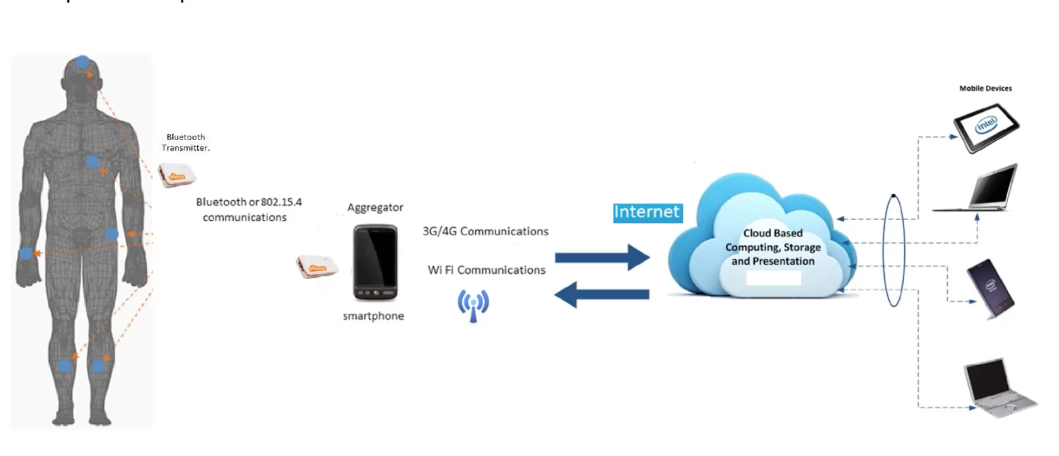
\includegraphics[scale=0.4]{imag/ArquitecturaREF.png}
\caption{Arquitectura de referencia. } %falta asignarREF
\label{10}
\end{figure}
\FloatBarrier

En el presente proyecto se desarrolló para el manejo de datos recibidos desde un dispositivo Android, una aplicación web donde se manejan el tipo de datos específicos de cada paciente y se encarga de monitorear el volumen respiratorio.

En esta aplicación web el fisioterapeuta puede registrar usuarios, asignar una prescripción por paciente, actualización de prescripciones y visualización de resultados del flujo respiratorio registrado de una fisioterapia respiratoria.




\subsection{Definición de Arquitectura para Sistema Web}

La siguiente arquitectura del sistema general siguiendo el modelado C4 para sistemas de software  definido para identificar y especificar los módulos y componentes del sistema web desde un primer nivel de abstracción.
%C1

\subsubsection{Diagrama contexto del sistema}

Dados las especificaciones de los servicios de fisioterapia y los requerimientos desarrollados se definen 3 módulos generales, representados en la figura \ref{11}, en este caso se presentan los sistemas que interactúan entre si y que componen el entorno general del proyecto. El módulo de \textit{aplicación de inspirómetro} en azul que se resalta para el manejo de las funcionalidades y las interacciones con el fisioterapeuta y los otros módulos de \textit{móvil} en gris e \textit{inspirómetro} como dispositivo médico:

\begin{figure}[ht]
\centering
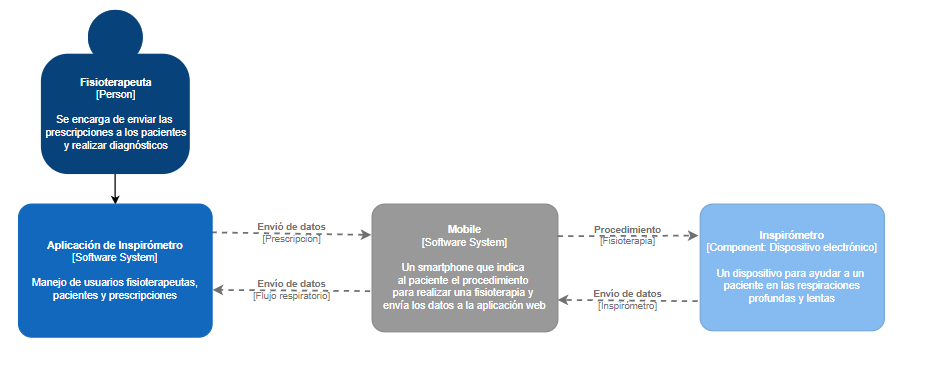
\includegraphics[scale=0.85]{imag/L1C4.PNG}
\caption{Diagrama contexto del sistema de fisioterapia respiratoria}
\label{11}
\end{figure}
\FloatBarrier

%C2
\subsubsection{Diagrama de contenedores}

Una vez se define el sistema web dentro de un entorno general, se expande el módulo de \textit{aplicación de inspirómetro} resalto en la figura \ref{11} anterior y se identifican funcionalidades especificas del sistema web como la interfaz de usuario y la base de datos. En este diagrama contenedor, la figura \ref{12} a continuación, se muestra las responsabilidades distribuidas en este componente, teniendo en cuenta también los módulos \textit{mobile} en gris e \textit{inspirómetro} para entender la comunicación entre ellos: 

\begin{figure}[ht]
\centering
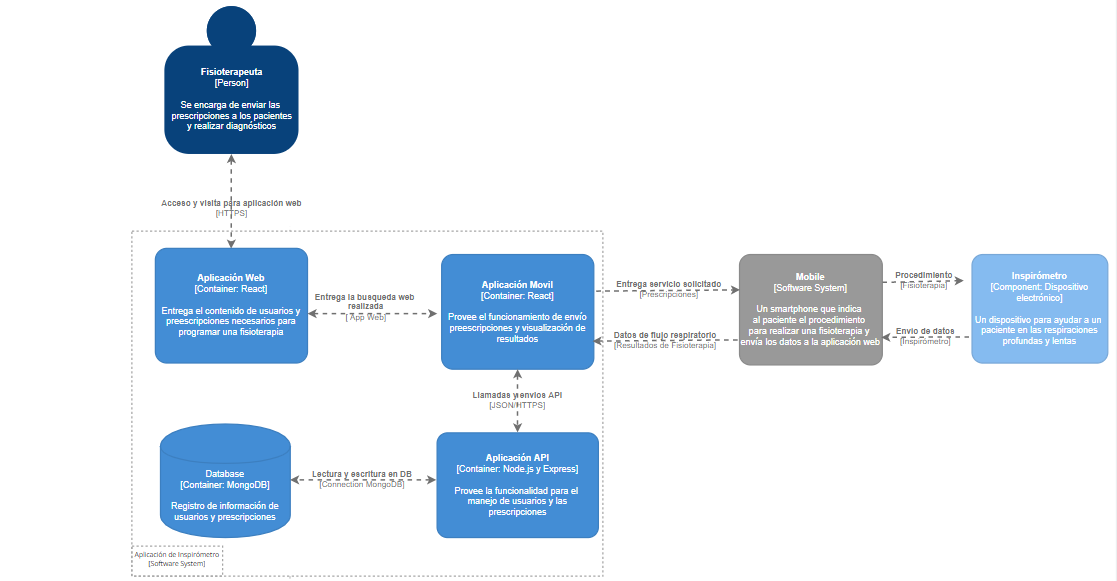
\includegraphics[scale=0.72]{imag/L2C4.PNG}
\caption{Diagrama de contenedores del sistema de fisioterapia respiratoria}
\label{12}
\end{figure}
\FloatBarrier

%C3
\subsubsection{Diagrama de componentes}

Se realiza una descomposición del módulo \textit{aplicación web} en la figura \ref{13}  y se identifican los componentes, ingreso a usuarios, lista de usuarios, seguridad, prescripciones y resultados que se van registrando en la base de datos. Por otro lado el sistema móvil y el componente de inspirómetro que son sistemas externos que envían los datos de flujo para ser visualizados en la aplicación web.

\begin{figure}[ht]
\centering
\includegraphics[scale=0.15]{imag/Untitled (2).png}
\caption{Diagrama de componentes del sistema de fisioterapia respiratoria}
\label{13}
\end{figure}
\FloatBarrier



%C4

\newpage

\subsubsection{Modelo de bases de datos}

Para la representación del modelo de datos del sistema se definen las clases de usuario a su vez asociadas las clases de paciente y fisioterapeuta, la clase de prescripción compuesta por la clase de usuario, puesto que una prescripción existe si un usuario existe, la relación entre estas dos clases es por cada usuario tenemos varias prescripciones, la clase de prescripción se compone también con la existencia de una clase ejercicios donde se encuentran establecidos los atributos que definen ese tipo de ejercicio, por último se encuentra la clase de resultados que depende de la clase ejercicios, pues estos resultados se asignan a el ejercicio que a su vez esta asignado a un usuario. A continuación en la figura \ref{14} se presenta el modelo de base de datos:


\begin{figure}[ht]
\centering
\includegraphics[scale=0.36]{imag/DB.png}
\caption{Modelo de Base de datos del sistema de fisioterapia respiratoria}
\label{14}
\end{figure}
\FloatBarrier


Este modelo representa cada uno de los tipos de datos y las dependencias desarrolladas para el sistema WEB-API.




\newpage

\section{Tecnologías de Implementación}

Para el desarrollo del sistema web se opta por utilizar React, conocido como una biblioteca de JavaScript para construir interfaces de usuario o creación de aplicaciones de front end, aprovechando el desarrollo basado en componentes es una característica que provee React y se utiliza en esta construcción de la interfaz de usuario. El desarrollo del banckend se realiza con Node.js, un entorno de ejecución para JavaScript multiplataforma que trabaja en tiempo de ejecución, se utiliza específicamente el framework de Node conocido como Express.js, que permite escritura de manejadores de peticiones con diferentes HTTP en diferentes rutas URL, en este caso Node facilita la transferencia de información o datos por que se escribe en JavaScript tanto del lado del servidor como del cliente. Para el manejo de datos se opta por utilizar MongoDB como complemento también para desarrollar en lenguajes basados en JavaScript como se puede ver en la figura \ref{15} de a continuación que representa las interacciones PUT, GET, POST, DELETE que son los métodos de HTTP de comunicación utilizados entre el server API y el sistema web, además de la relación representa QUERY y RESULT con la base de datos:

%REACT
%C1
\begin{figure}[ht]
\centering
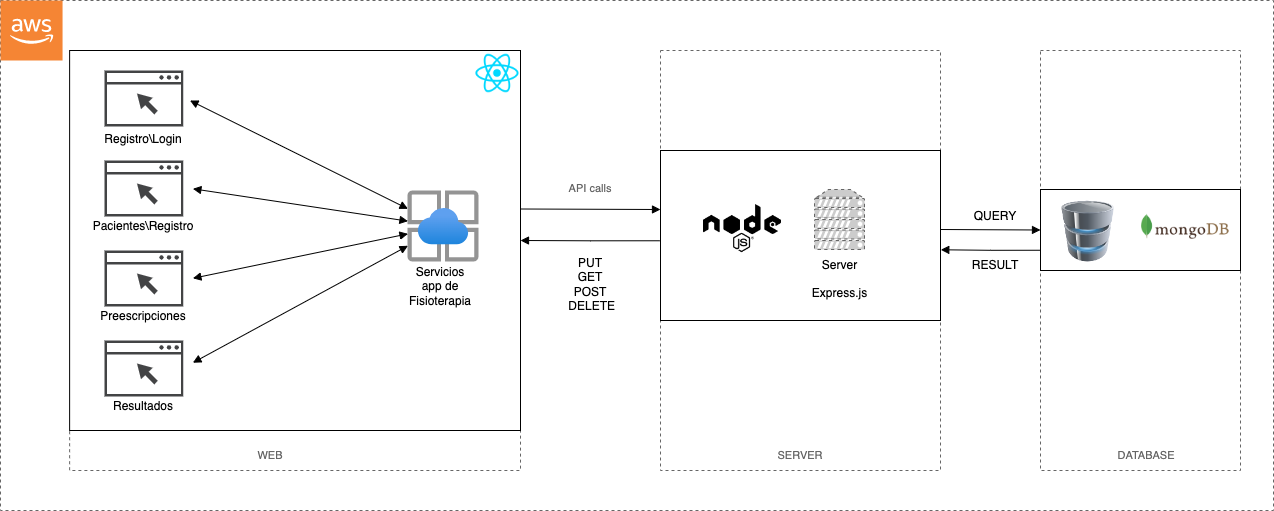
\includegraphics[scale=0.4]{imag/ArquAWS.png}
\caption{Arquitectura de aplicación web }
\label{15}
\end{figure}
\FloatBarrier

Para el despliegue del sistema web en la nube se opta por utilizar AWS que permite el almacenamiento, mantenimiento de servidores y el acceso a bases de datos establecidas, el diagrama de a continuación de la figura \ref{16} muestra el flujo del despliegue de la información, contando con una instancia Lightsail de AWS donde se encuentra el sistema web que proporciona el sitio web del mismo.

\begin{figure}[ht]
\centering
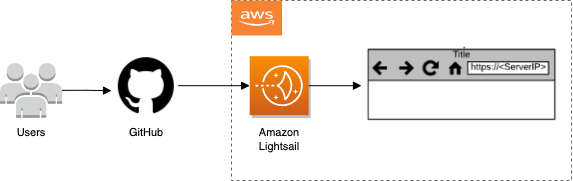
\includegraphics[scale=0.45]{imag/Lightsail.png}
\caption{Arquitectura de despliegue del sistema web }
\label{16}
\end{figure}
\FloatBarrier


Las tecnologías web de implementación utilizadas JavaScript y React son las más utilizadas para desarrollo web en la actualidad por que permiten la creación de animaciones, formularios, desarrollo basado en componentes y distintos elementos web, también se utiliza para del servidor API, Node.js que permite construir aplicaciones de red que son compatibles con plataformas en Linux, SunOS, Mac OS X y Windows \cite{52} \cite{53}.






\subsection{API}

Se implementó el proyecto API con los servicios de comunicación que se definieron en base a los requerimientos priorizados, se utiliza en este caso Postman la herramienta que permite realizar pruebas API,  se describen a continuación: 


\subsubsection{Comunicación local entre aplicación Web y API}

\begin{enumerate}
    \item \textbf{Servicio de autenticación:} 
    Se crea el servicio \textit{authenticateUser} que permite el acceso a la información de los datos del usuario, en este caso, el usuario tipo fisioterapeuta y tipo paciente, con la petición en el ejemplo de a continuación se obtiene el token de validación, el cual sera necesario para acceder a los otros servicios que requieren autorización como se muestra en la figura \ref{17}:
           
            \begin{figure}[ht]
            \centering
            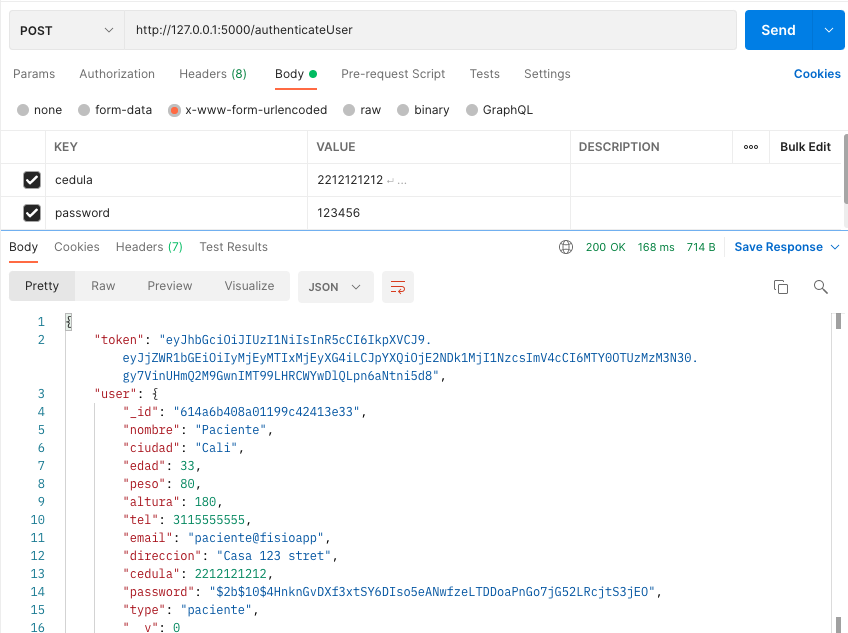
\includegraphics[scale=0.35]{imag/pacienteau.png}
            \caption{Petición HTTP post en Postman de autenticación de usuario paciente}
            \label{17}
            \end{figure}
            \FloatBarrier
            
    \item \textbf{Servicio de consulta a todos los pacientes:} 
    Se crea el servicio \textit{allUsers} para obtener el id del usuario del cual se requiere consultar su prescripción, la prueba consiste en llamar este servicio enviando el token obtenido en el paso anterior como se muestra en la figura \ref{18}:
    
            \begin{figure}[ht]
            \centering
            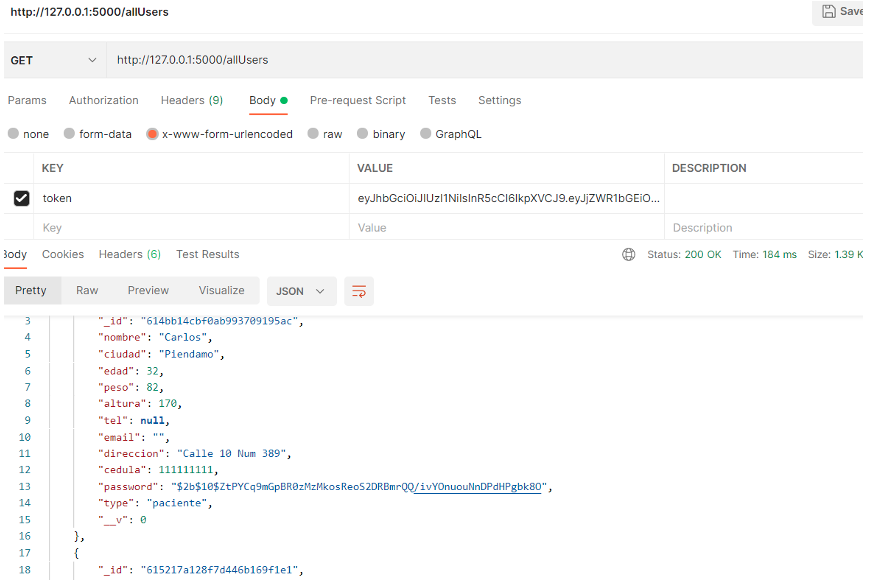
\includegraphics[scale=0.35]{imag/allus.png}
            \caption{Petición GET en Postman para ver todos los usuarios }
            \label{18}
            \end{figure}
            \FloatBarrier
            
    \item \textbf{Servicio de prescripción:}
    Para obtener la prescripción de un paciente donde se muestran los ejercicios recomendados se crea el servicio \textit{allEjerciciosByUser}, para la prueba se hace el llamado al servicio enviando los datos como se muestran en el siguiente ejemplo. El resultado muestra los datos de la prescripción para el paciente, el campo que esta marcado como null, no es considerado para ningún efecto. En este caso en particular el token se programó para expirar en 3 horas si no se hace ninguna petición en este lapso como se muestra en la figura \ref{19}:
    
            \begin{figure}[ht]
            \centering
            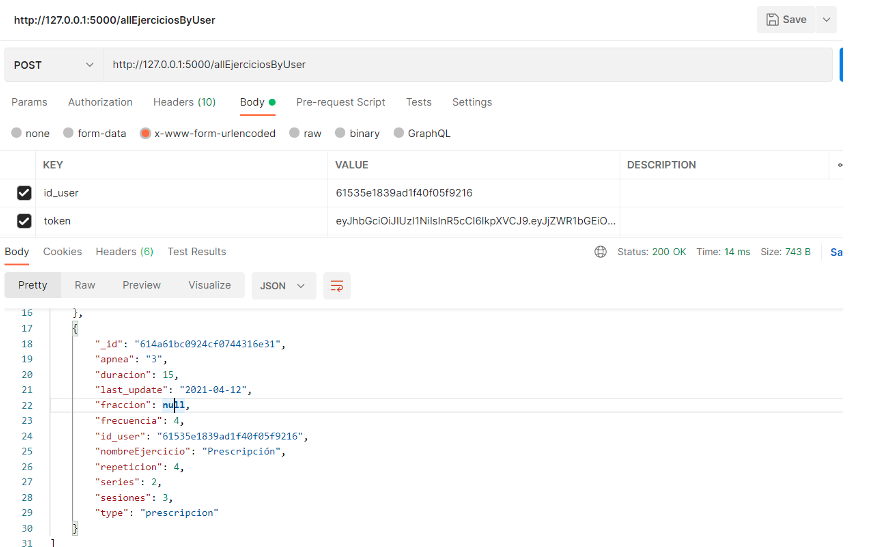
\includegraphics[scale=0.35]{imag/prees.png}
            \caption{Petición POST en Postman para ver prescripción de paciente }
            \label{19}
            \end{figure}
            \FloatBarrier
            
            
    \item \textbf{Servicio para cargar resultados del paciente:} Se crea el servicio \textbf{createResult}.Este servicio permite la carga de los resultados obtenidos con el dispositivo smarthphone donde se realizó la fisioterapia respiratoria. Este servicio se implementan con la posibilidad de crear resultados ya sea por paciente o de todos los pacientes, teniendo en cuenta la relación existente entre el id del ejercicio y el id user, como también con la posibilidad de obtener todos los resultados de los pacientes como se muestra en la figura \ref{20}, \ref{21} y \ref{22}:
    
            \begin{figure}[ht]
            \centering
            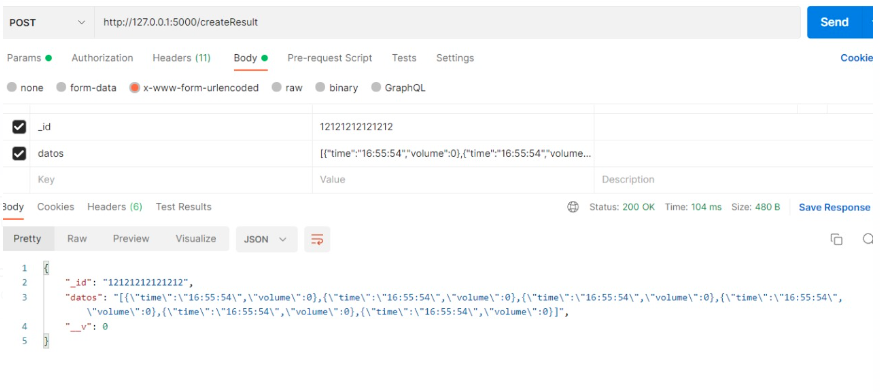
\includegraphics[scale=0.3]{imag/createresult.png}
            \caption{Petición POST en Postman para cargar un resultado de un paciente }
            \label{20}
            \end{figure}
            \FloatBarrier
            
            
            \begin{figure}[ht]
            \centering
            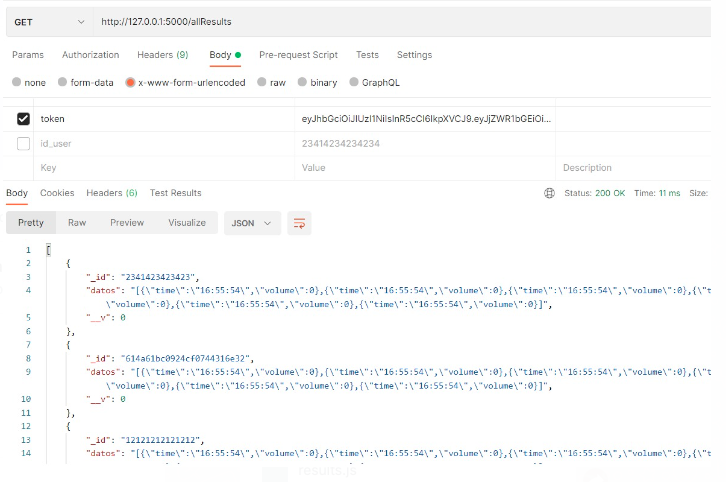
\includegraphics[scale=0.3]{imag/allresults.png}
            \caption{Petición GET en Postman para ver todos los resultados }
            \label{21}
            \end{figure}
            \FloatBarrier
            
            
            \begin{figure}[ht]
            \centering
            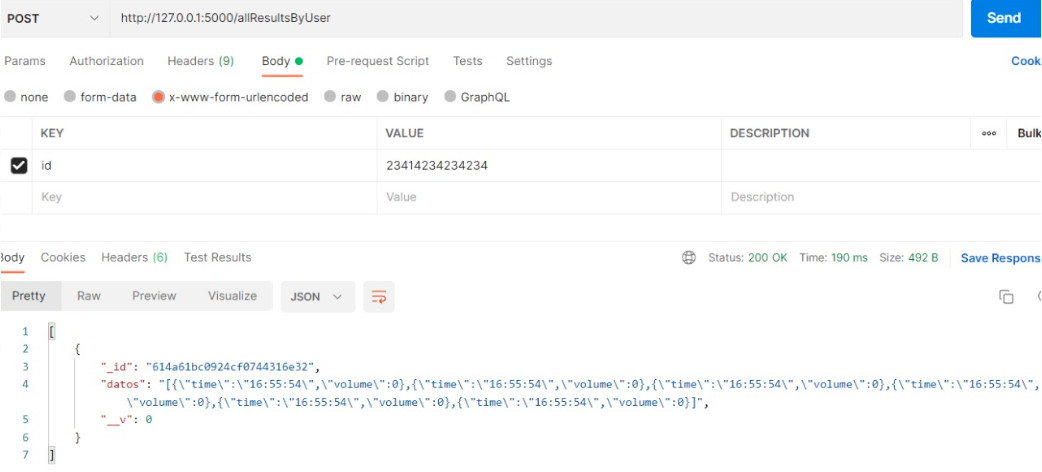
\includegraphics[scale=0.25]{imag/resultsbyuser.png}
            \caption{Petición POST en Postman para cargar todos los resultados }
            \label{22}
            \end{figure}
            \FloatBarrier
    
    
\end{enumerate}



\newpage

\subsection{Servidor Virtual}

Para dejar el proyecto API en la nube y tener la url publica para el acceso del usuario final, se crea el servidor virtual en AWS lightsail, lo cual es una herramienta que brinda la creación y gestión de instancias para aplicaciones web. En este caso contamos con dos instancias una para la base de datos y otra para la aplicación como se muestra en la figura \ref{23}:.

\begin{figure}[ht]
\centering
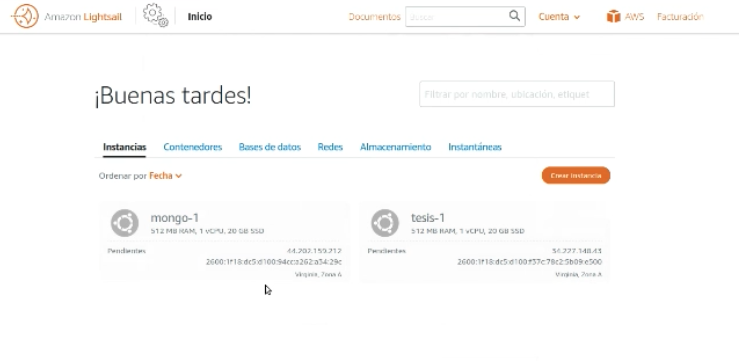
\includegraphics[scale=0.4]{imag/maquinasAWS.png}
\caption{Creación de instancias en AWS }
\label{23}
\end{figure}
\FloatBarrier


Por lo tanto, se puede gestionar como una red virtual privada para que la aplicación web se conecte con la base de datos y se pueda gestionar su acceso mediante la vinculación con una IP estática como se muestra en la figura \ref{24}: 

\begin{figure}[ht]
\centering
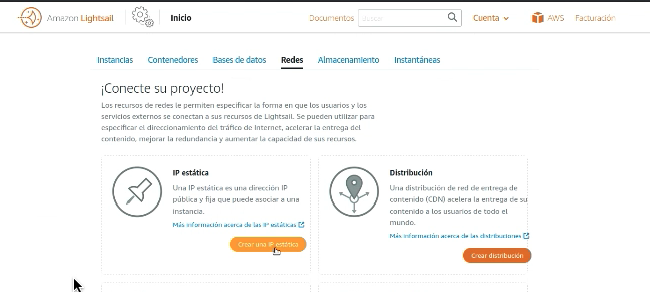
\includegraphics[scale=0.4]{imag/IPestaticaAWS.png}
\caption{Vinculación IP estática }
\label{24}
\end{figure}
\FloatBarrier


La instancia para el proyecto software de fisioterapia respiratorio que incluye un proyecto de desarrollo web y un API quedó definido como se muestra en la figura \ref{25}:

\begin{figure}[ht]
\centering
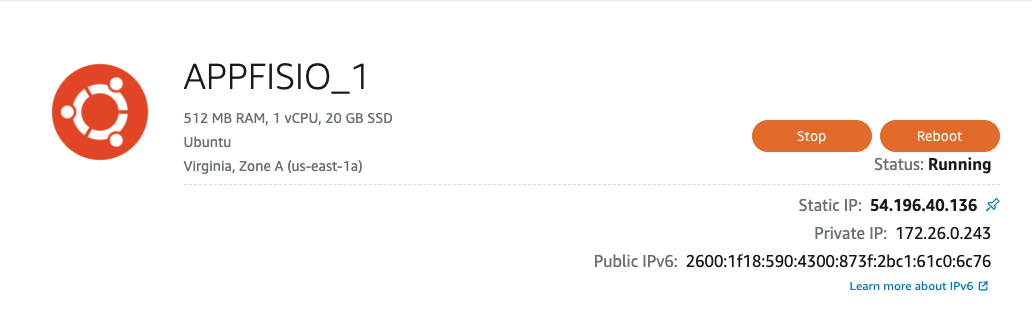
\includegraphics[scale=0.4]{imag/instanciafisio.png}
\caption{Instancia para el proyecto de software de fisioterapia}
\label{25}
\end{figure}
\FloatBarrier







\subsection{Comunicación online entre aplicación Web y API}

Gracias a la creación de la instancia del proyecto API en AWS se logra el manejo de servicios en la nube, el proyecto API disponible en \url{https://d2yaaz8bde1qj3.cloudfront.net/} que permite la disponibilidad de los servicios desarrollados y que pueden ser consumidos según sea la gestión de este recurso. 

\textit{ \textbf{Nota:} Tener en cuenta que el alcance del proyecto es un prototipo, por lo tanto, el software API se encuentra desplegado en un servidor privado que necesita de su activación por parte del administrador del sistema antes de su consumo.}

A continuación se presentan los servicios desarrollados que se pueden consultar en la herramienta Postman utilizando la dirección https generada.


\begin{enumerate}
    \item \textbf{Servicio de autenticación online:} Autenticarse en el API, el usuario valido es el usuario con los siguientes datos como se muestra en la figura \ref{26}:

            \begin{figure}[ht]
            \centering
            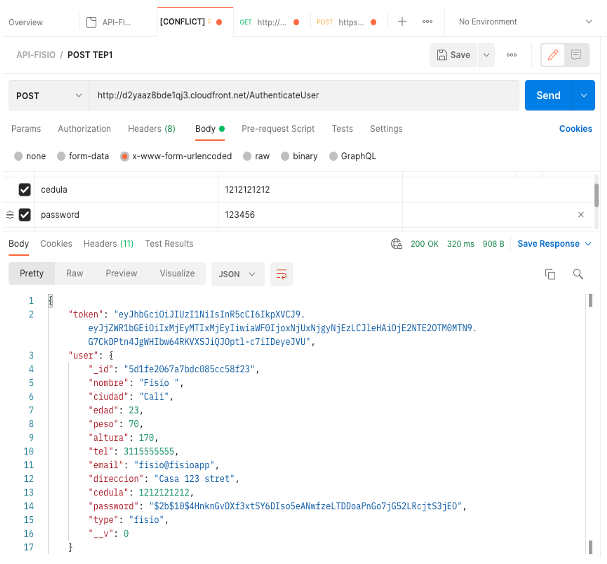
\includegraphics[scale=0.3]{imag/authuseronline2.png}
            \caption{Petición http post en Postman de autenticación de usuario }
            \label{26}
            \end{figure}
            \FloatBarrier
    Con esta petición se obtiene el token, el cual será necesario para acceder a los otros servicios que requieren autorización.
            
\newpage
            
    \item \textbf{Servicio de consulta a todos los pacientes online:} 
    
            \begin{figure}[ht]
            \centering
            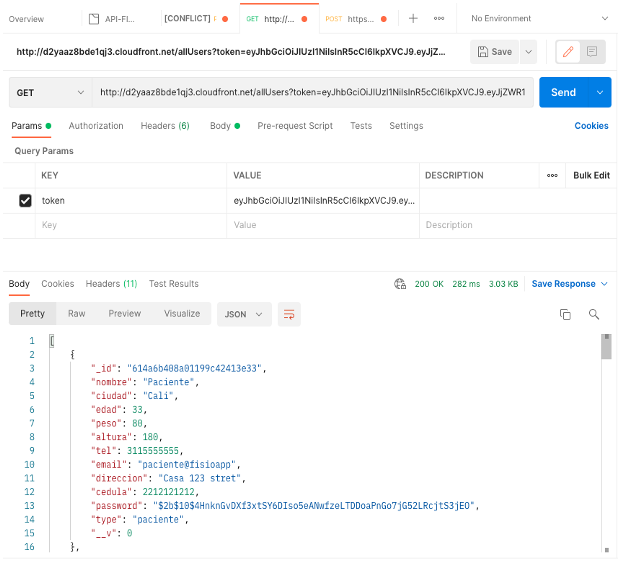
\includegraphics[scale=0.35]{imag/allusersonline.png}
            \caption{Petición get en Postman para ver todos los usuarios }
            \label{27}
            \end{figure}
            \FloatBarrier
            
    \item \textbf{Servicio de prescripción online:}
    
            \begin{figure}[ht]
            \centering
            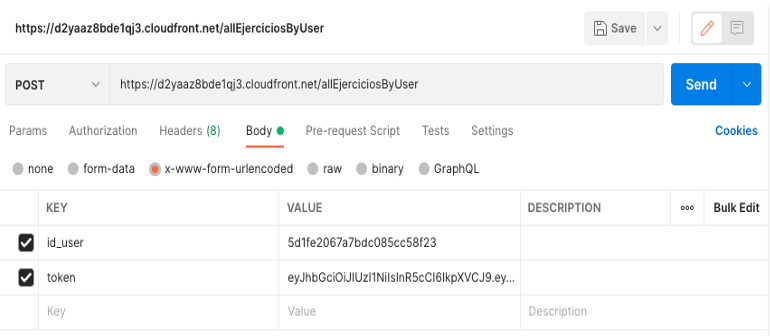
\includegraphics[scale=0.35]{imag/presonline2.png}
            \caption{Petición post en Postman para ver prescripción de paciente }
            \label{28}
            \end{figure}
            \FloatBarrier
            
    \item \textbf{Servicio para crear un usuario:}
    Para crear un usuario que se va a registrar en la aplicación es necesario tener en cuenta revisar el servicio allUsers para no repetir la cédula, dado a que es un campo obligatorio que se va validar como se muestra en la figura \ref{29}: 
    
            \begin{figure}[ht]
            \centering
            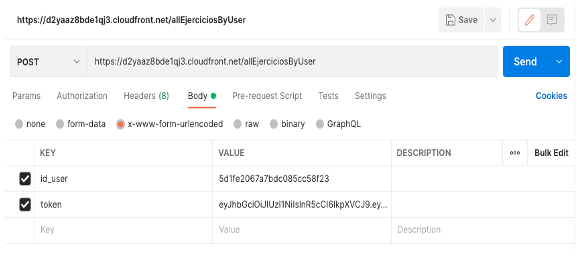
\includegraphics[scale=0.5]{imag/presonline.png}
            \caption{Petición post en Postman para la creación de un paciente }
            \label{29}
            \end{figure}
            \FloatBarrier
    
    

            
    \item \textbf{Servicio para cargar resultados del paciente:}
    
    Para el envió de los resultados del paciente se requiere preferiblemente la generación de un archivo json por medio de una url para ser leida desde la aplicación como se muestra en la figura \ref{30}, \ref{31} y \ref{32}:
   
    
            \begin{figure}[ht]
            \centering
            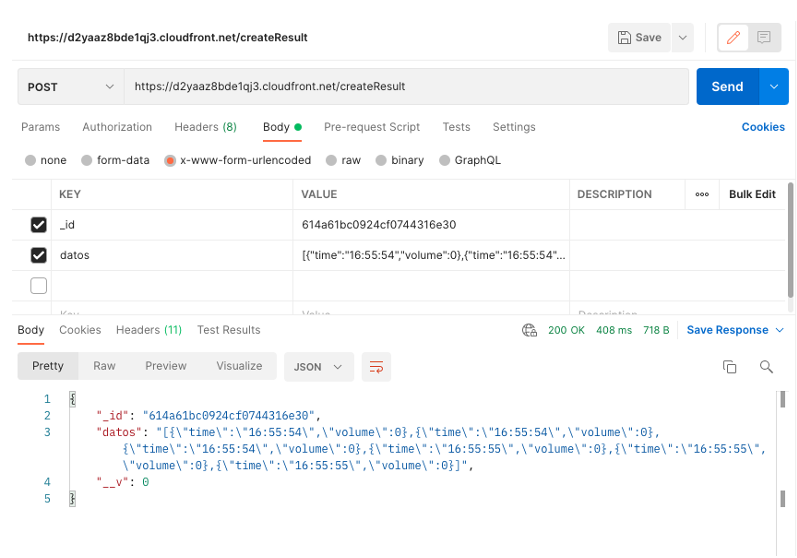
\includegraphics[scale=0.35]{imag/createresultonline.png}
            \caption{Petición post en Postman para cargar un resultado de un paciente }
            \label{30}
            \end{figure}
            \FloatBarrier
            
            
            \begin{figure}[ht]
            \centering
            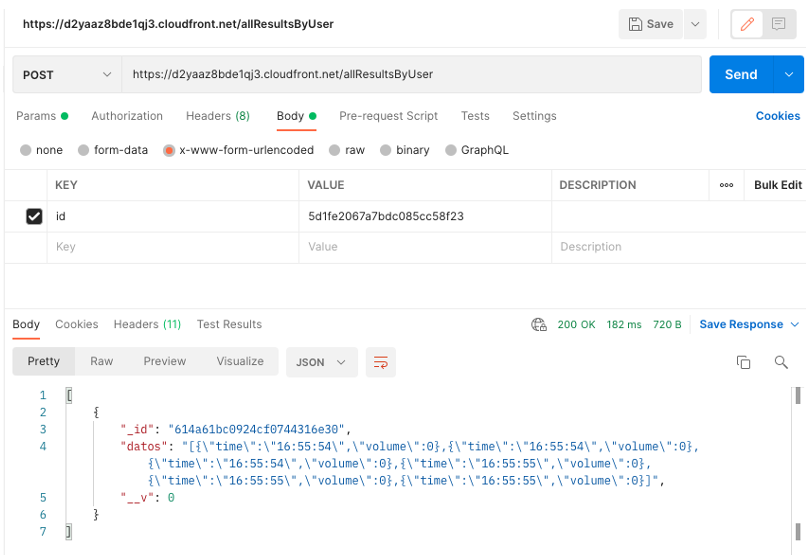
\includegraphics[scale=0.35]{imag/allresultsbyuseronline.png}
            \caption{Petición post en Postman para cargar todos los resultados }
            \label{31}
            \end{figure}
            \FloatBarrier
            
            \begin{figure}[ht]
            \centering
            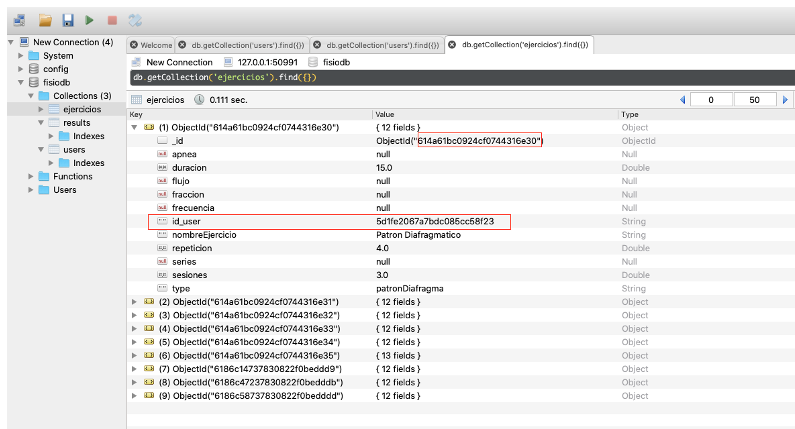
\includegraphics[scale=0.4]{imag/realcionmongoonline.png}
            \caption{Configuración en mongo entre el id de usuario y ejercicio }
            \label{32}
            \end{figure}
            \FloatBarrier
            
            
    
    
\end{enumerate}













%\subsection{Peticiones web con nodemon}



%prototipos iniciales del sistema





\newpage
\section{Aplicación Web}

En esta sección se explica las utilidades de React para el desarrollo de la interfaz de usuario del sistema software de fisioterapia.

La aplicación web es desarrollada bajo los conceptos de Semantic UI, framework para crear diseños de interfaces de manera responsive utilizando HTML y CSS que permite la creacion de componentes React, HTML para la creación de formularios y CSS para el estilo de cada página web \cite{33}.


\subsection{Funciones de React}

A continuación se describen las funciones de React y NodeJS que se utilizaron en el desarrollo del sistema web:

\begin{itemize}
    \item \textbf{Controlers:} Tanto en la aplicación web como para el desarrollo de un API REST con NodeJS se permite la función de componentes controlados, especialmente para el desarrollo del API se desarrollan controladores y rutas que toman las acciones especificadas en la codificación.
    \item \textbf{Reducers:} Redux conocido como un contendedor predecible del estado de aplicaciones JavaScript \cite{34}. Su uso en React para permitir describir la interfaz de usuario como una función de estado, es decir emite actualizaciones de estado en respuesta a acciones. 
    \item \textbf{Routers:} Como conjunto de componentes de navegación que se utilizaron en la aplicación web y por lo cual se permitió establecer rutas como: home, inicio de sesión, etc. como también la realización de redirecciones a otras paginas según ciertas condiciones \cite{35}.
    \item \textbf{Models:} esta función utilizada para el desarrollo del backend de la aplicación web. Se crean modelos y entidades en NodeJS que van a representar a una entidad en la base de datos y mas concretamente a un único registro o documento de la base de datos.
    
    
\end{itemize}




\subsection{Prototipo Funcional del Sistema Web }

En esta sección se presenta el prototipo funcional del sistema donde se especifica en detalle las funcionalidades

\subsubsection{Inicio de sesión para usuarios}

El usuario tanto paciente como fisioterapeuta respiratorio cuenta con el ingreso de sesión como se muestra en la figura \ref{33}:

\begin{figure}[ht]
\centering
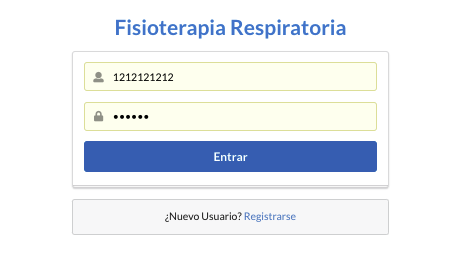
\includegraphics[scale=0.6]{imag/appiniciosesion.png}
\caption{Inicio de sesión}
\label{33}
\end{figure}
\FloatBarrier


\subsubsection{Lista de usuarios}

El fisioterapeuta tiene fijada una lista de pacientes que se presenta por cédula y por nombre, en esta vista de la interfaz, el fisioterapeuta puede ver la prescripción del paciente seleccionado, eliminar o registrar un paciente ver su prescripción como se muestra en la figura donde se tienen usuarios de prueba registrados \ref{34}:

\begin{figure}[ht]
\centering
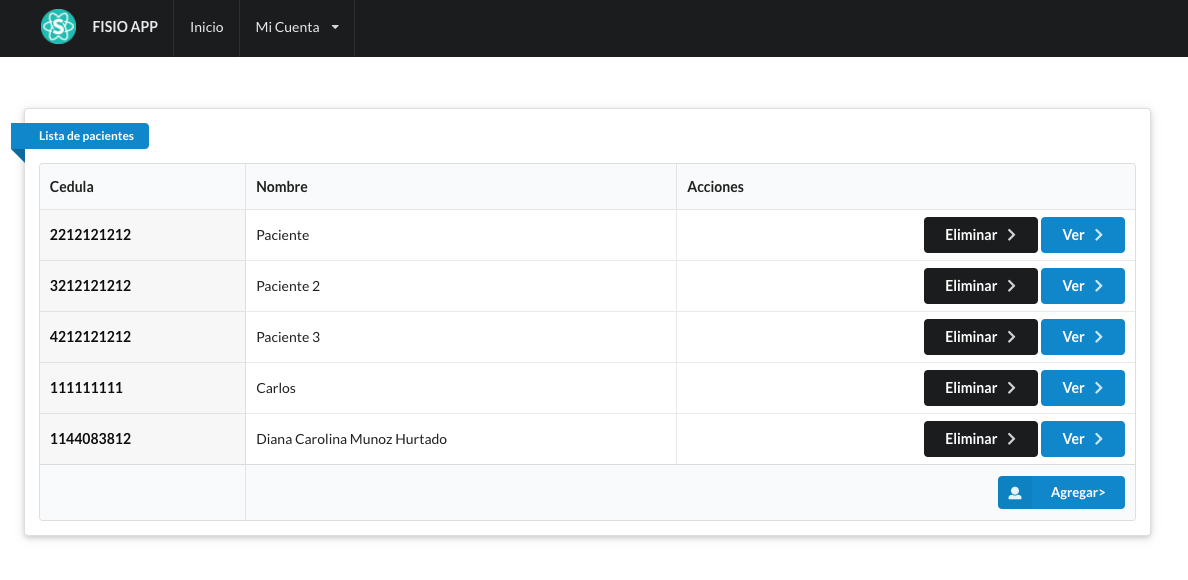
\includegraphics[scale=0.3]{imag/listpacientes.png}
\caption{Lista de pacientes}
\label{34}
\end{figure}
\FloatBarrier

Para registrar un nuevo paciente se requiere los datos que se muestran a continuación en la figura \ref{35}, donde es importante definir también el tipo de usuario ya sea paciente o fisioterapeuta:

\begin{figure}[ht]
\centering
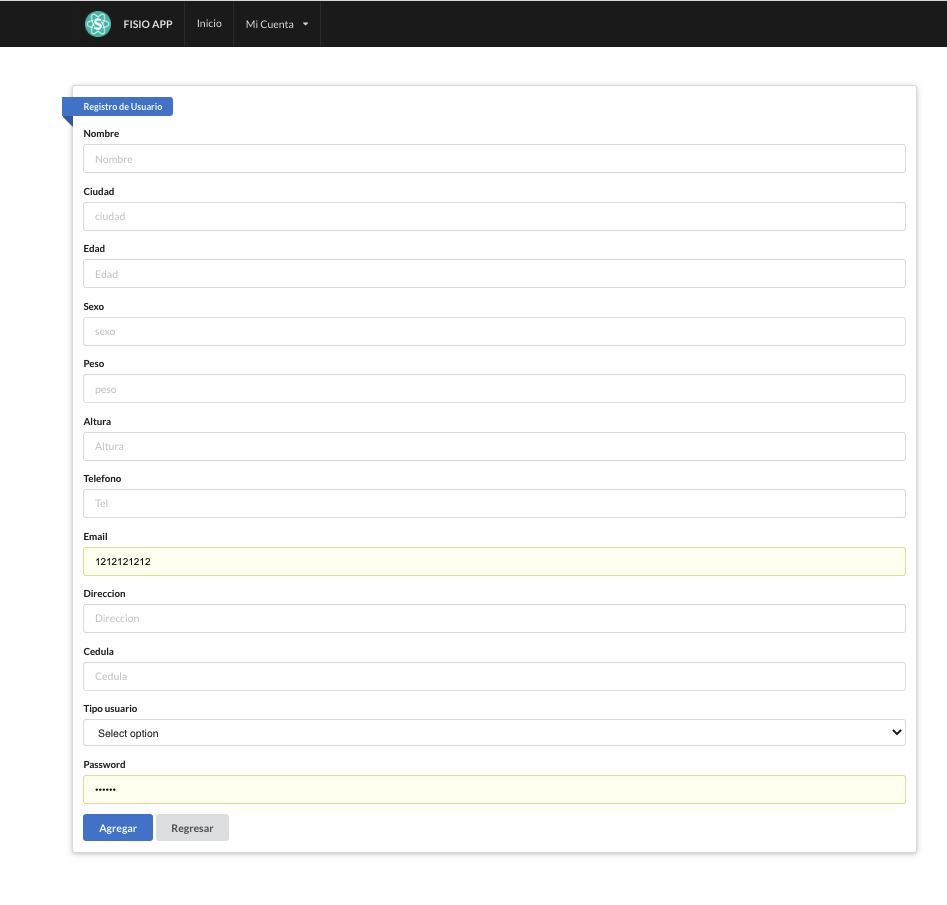
\includegraphics[scale=0.5]{imag/appregistrousuario.png}
\caption{Registro de pacientes}
\label{35}
\end{figure}
\FloatBarrier

\subsubsection{Información de pacientes}

Se despliega la información de los pacientes, con la opción de cargar una imagen personalizada previamente disponible, en esta ventana encuentra la opción de ver las prescripciones asignadas y agregar una nueva, como se muestra en la figura \ref{36}:


\begin{figure}[ht]
\centering
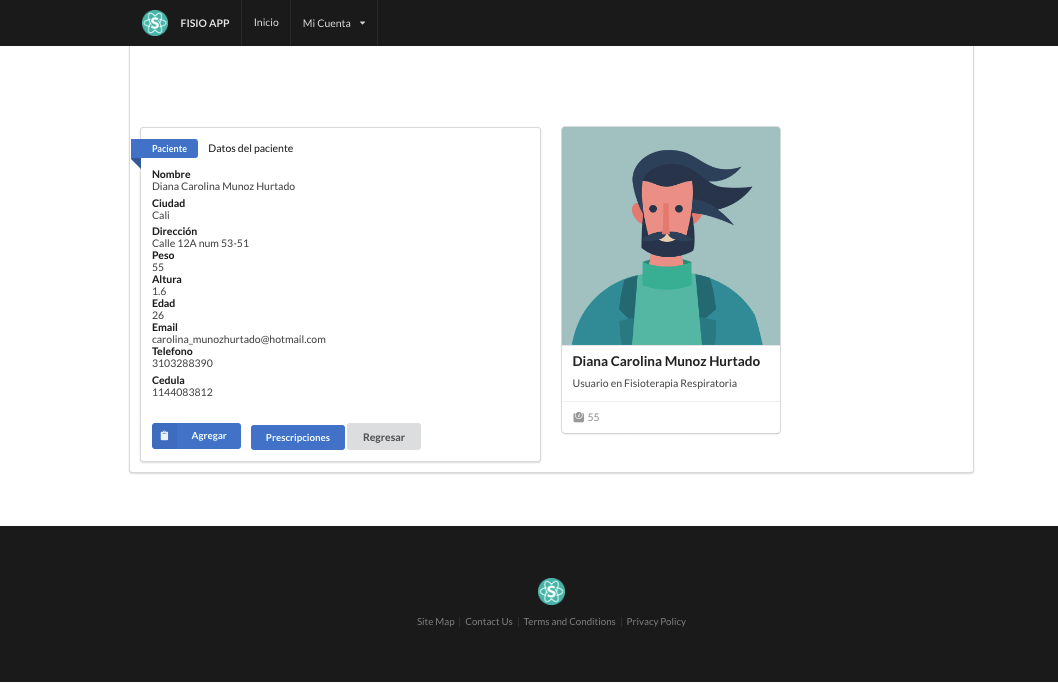
\includegraphics[scale=0.3]{imag/appverdatosusuarios2.png}
\caption{Datos del paciente}
\label{36}
\end{figure}
\FloatBarrier

En la ventana anterior en la opción agregar puede agregar la prescripción que necesita registrar con los datos necesarios como se muestra en la figura \ref{37}:


\begin{figure}[ht]
\centering
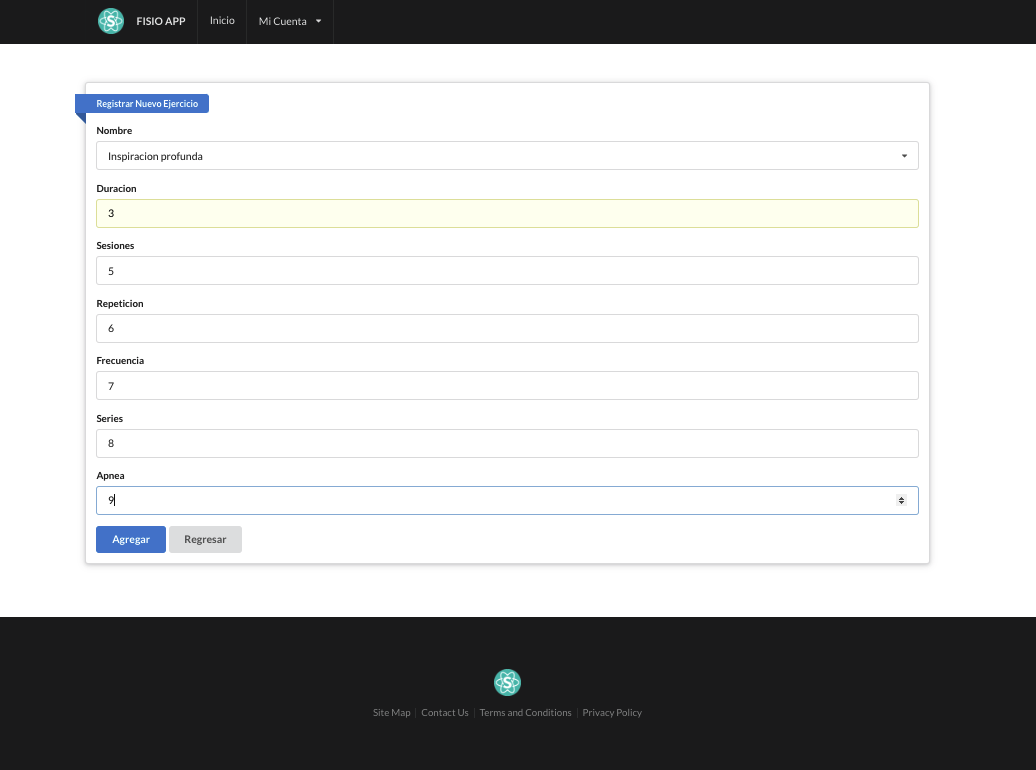
\includegraphics[scale=0.3]{imag/appregistrarpreescripcion.png}
\caption{Registrar una prescripción}
\label{37}
\end{figure}
\FloatBarrier


En la prescripción del paciente el fisioterapeuta podrá ver para el paciente seleccionado, la capacidad vital calculada por el sistema dados los datos del paciente, también puede ver los indicadores de fisioterapia que han sido asignados al paciente previamente en la figura \ref{38}:

\begin{figure}[ht]
\centering
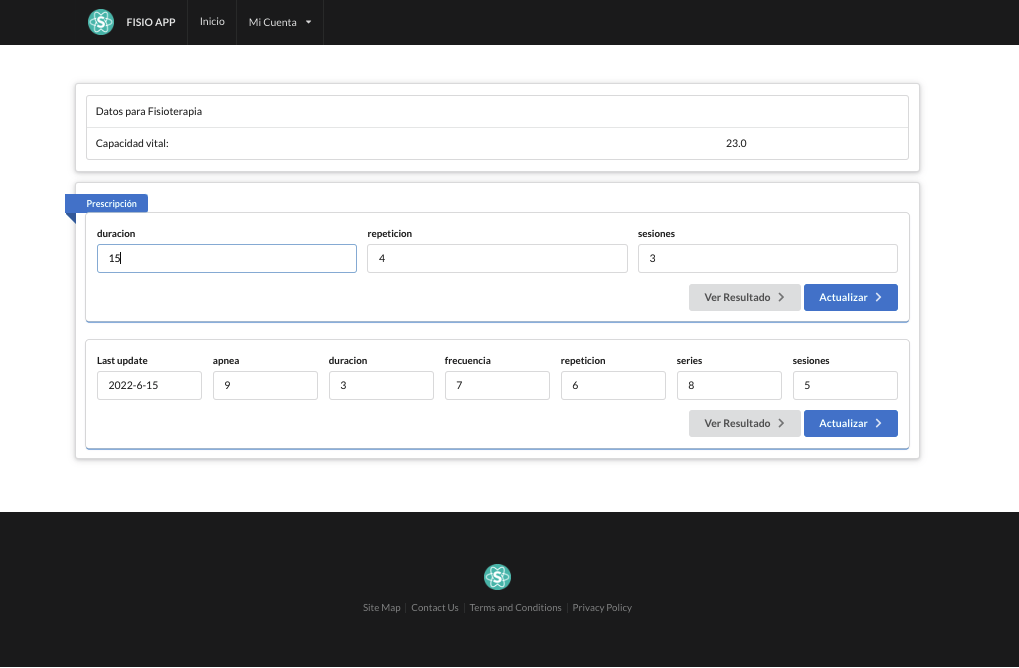
\includegraphics[scale=0.3]{imag/appprescripcionuser.png}
\caption{Prescripción asignada a un paciente}
\label{38}
\end{figure}
\FloatBarrier



\subsubsection{Visualización de resultados}

Para cada uno de las prescripciones realizadas el fisioterapeuta respiratorio tiene la posibilidad de ver el comportamiento de los resultados mediante la gráfica presentada con la opción \textit{ver resultados} en la figura \ref{39} se puede observar dos gráficas, la primera de flujo que representa los datos recibidos desde el sistema móvil que previamente ya procesó antes de su envío, la segunda gráfica de volumen, que se calcula a partir de los datos de flujo entregados. Para el cálculo de los datos de volumen se realiza una suma con los datos de flujo, como se puede ver en el ejemplo \ref{vol}:

\begin{figure}[ht]
\centering
\includegraphics[scale=0.5]{imag/datosgv.png}
\caption{Ejemplo de cálculo de los datos de volumen}
\label{vol}
\end{figure}
\FloatBarrier




También se puede observar que la visualización permite conocer cada uno de los puntos de la gráfica con el marcador de referencia que se presenta cuando se recorre la gráfica :

\begin{figure}[ht]
\centering
\includegraphics[scale=0.3]{imag/datosvisuales.png}
\caption{Visualización de flujo respiratorio}
\label{39}
\end{figure}
\FloatBarrier




 \subsection{Pruebas del sistema web}
 
\subsubsection{Prueba de validación de envío de datos por paciente }
Con el objetivo de comprobar el procedimiento de carga de resultados por paciente desarrollado, en esta prueba se valida el flujo de envío de datos hasta lograr la visualización de las gráficas de los resultados en la aplicación web como se observa en la figura \ref{40}:

Se valida la existencia del usuario tipo paciente en la plataforma:
\begin{figure}[ht]
\centering
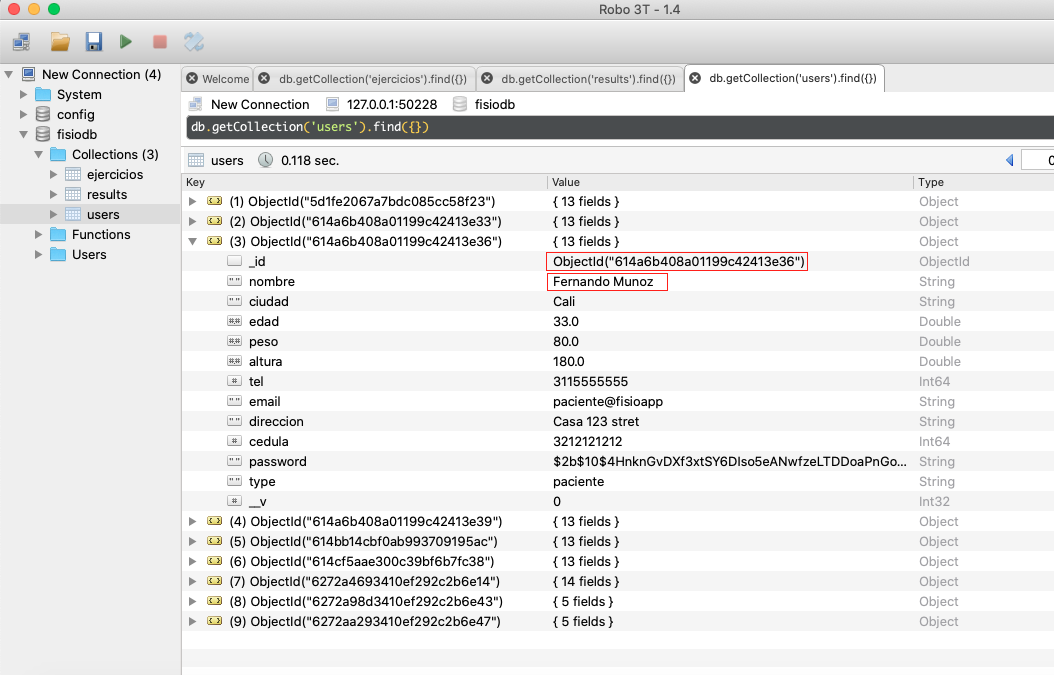
\includegraphics[scale=0.3]{imag/TEST1User.png}
\caption{Validación de usuarios en base de datos}
\label{40}
\end{figure}
\FloatBarrier

En la base de datos, en la colección de ejercicios, se valida que el usuario tipo paciente tenga asignado un ejercicio en la figura \ref{41}:

\begin{figure}[ht]
\centering
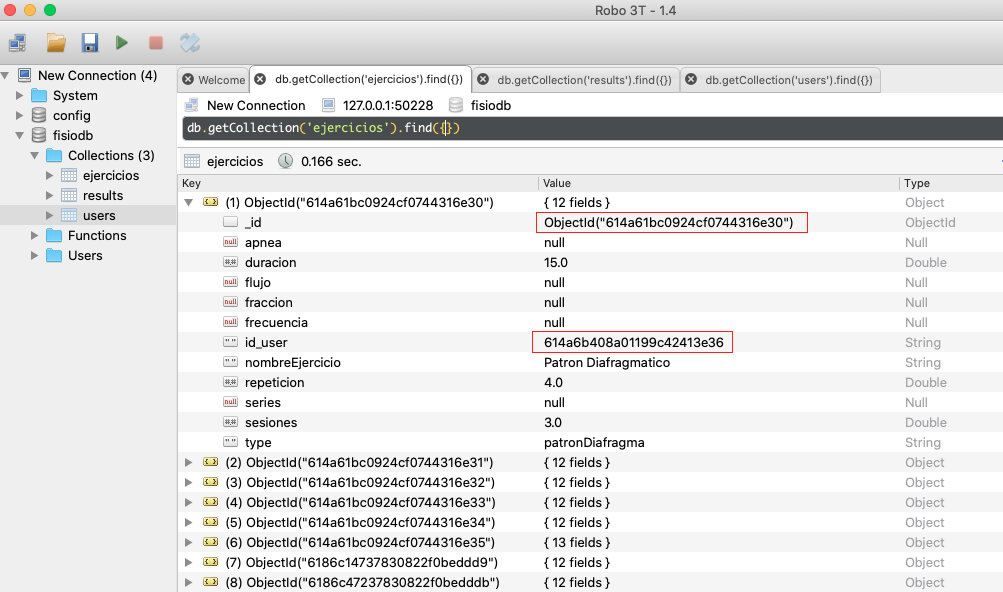
\includegraphics[scale=0.3]{imag/TEST2Ejercicio.png}
\caption{Validación de ejercicios en base de datos}
\label{41}
\end{figure}
\FloatBarrier

Desde la herramienta Postman que permite la carga de los resultados de prueba, se valida que el envío de datos sea satisfactorio como se observa en la figura \ref{42}:

\begin{figure}[ht]
\centering
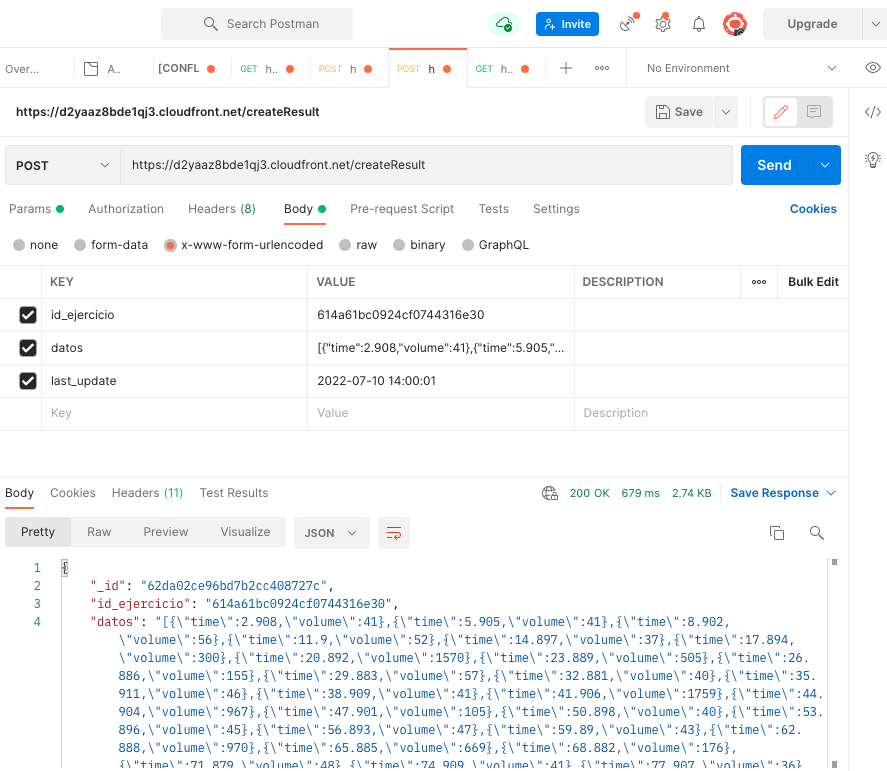
\includegraphics[scale=0.3]{imag/TEST3sendData.png}
\caption{Validación de envío de datos}
\label{42}
\end{figure}
\FloatBarrier

Se valida que la carga de resultados se actualice en la base de datos como se observa en la figura \ref{43}:

\begin{figure}[ht]
\centering
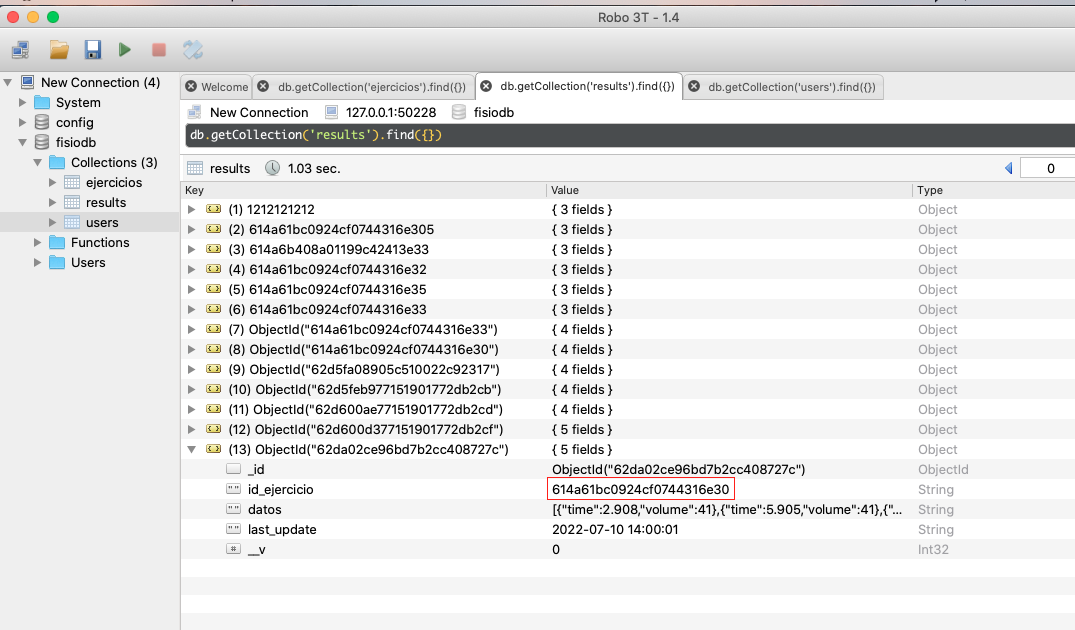
\includegraphics[scale=0.3]{imag/TEST4Results.png}
\caption{Validación de carga de resultados }
\label{43}
\end{figure}
\FloatBarrier

Se realiza doble verificación en la consola del servidor en web como se observa en la figura \ref{44}:

\begin{figure}[ht]
\centering
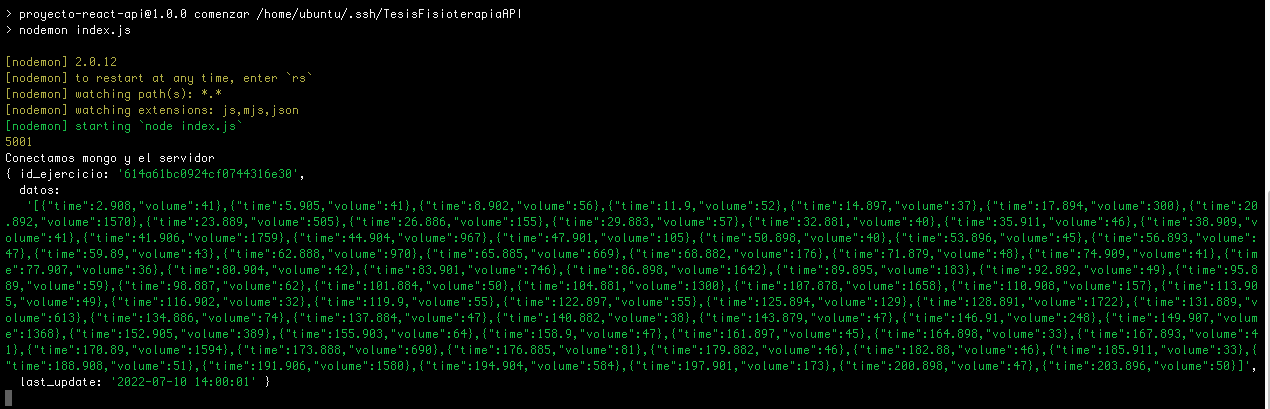
\includegraphics[scale=0.3]{imag/TEST5Console.png}
\caption{Validación de datos en servidor web}
\label{44}
\end{figure}
\FloatBarrier

Desde la aplicación web, ingresamos a validar estos datos del usuario tipo paciente seleccionado inicialmente como se observa en la figura \ref{45}::

\begin{figure}[ht]
\centering
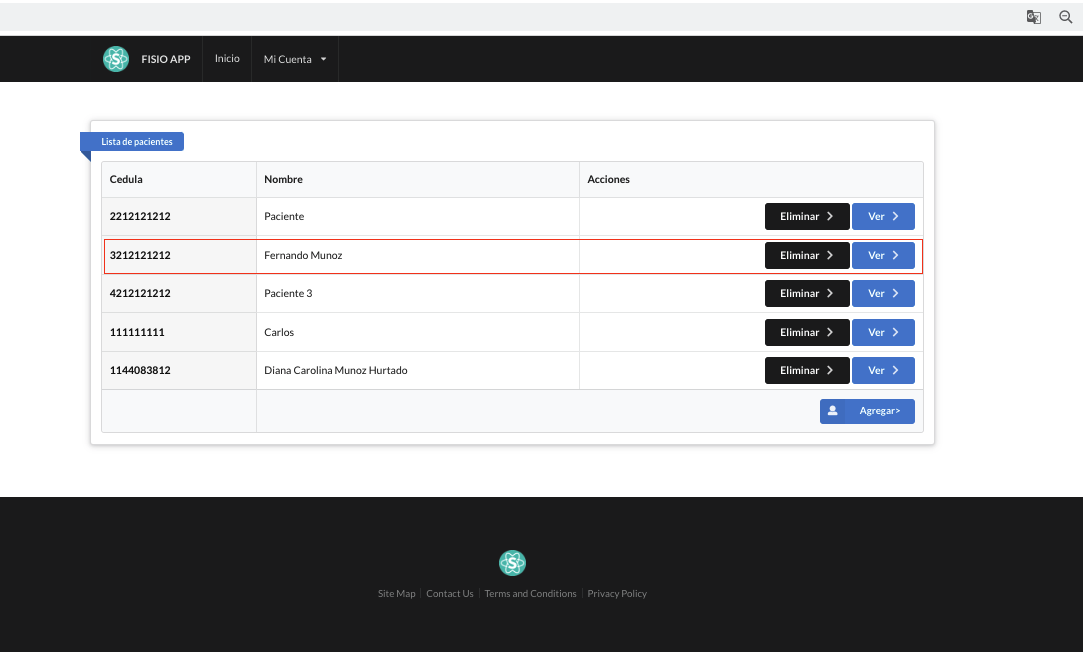
\includegraphics[scale=0.3]{imag/TEST6UserF.png}
\caption{Validación de usuarios en aplicación web }
\label{45}
\end{figure}
\FloatBarrier

Se presenta la prescripción asignada al paciente con fecha y hora de la data enviada inicialmente como se observa en la figura \ref{46}:

\begin{figure}[ht]
\centering
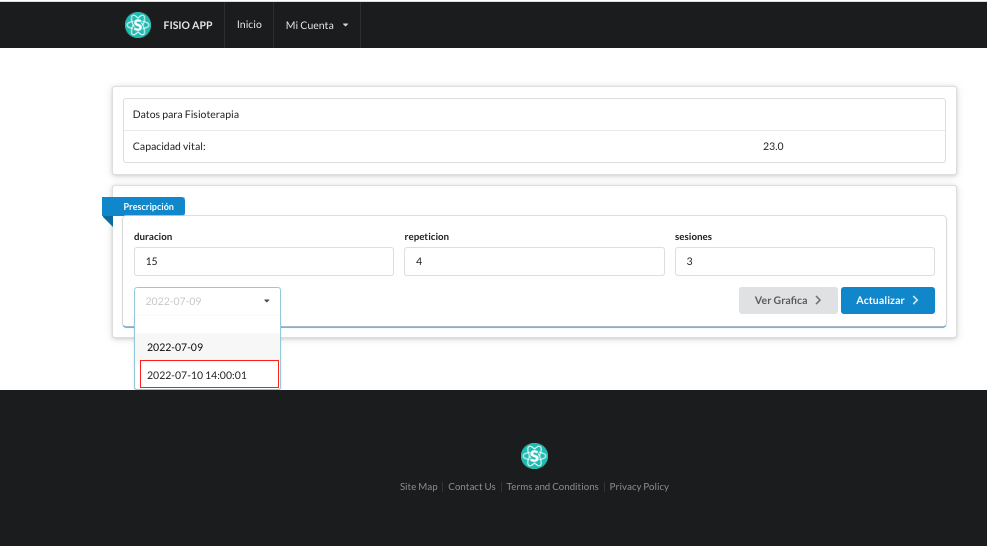
\includegraphics[scale=0.3]{imag/TEST7Preescrip.png}
\caption{Validación de datos de prescripción }
\label{46}
\end{figure}
\FloatBarrier



Finalmente las gráficas flujo y volumen de resultados enviados al paciente como se observa en la figura \ref{47}:

\begin{figure}[ht]
\centering
\includegraphics[scale=0.3]{imag/TEST8Graficas.png}
\caption{Validación de resultados }
\label{47}
\end{figure}
\FloatBarrier


\subsubsection{Prueba de validación de conexión envío de datos por paciente con el sistema móvil }

A continuación en la figura \ref{48}, \ref{49}, \ref{50} y \ref{51} la prueba realizada con la conexión del sistema móvil encargado del recibimiento de las prescripciones y el envió de resultados al paciente: 

Inicio del sistema móvil para fisioterapia:

\begin{figure}[ht]
\centering
\includegraphics[scale=0.3]{imag/TESTseleccionejericiomobile.png}
\caption{Inicio de fisioterapia desde sistema móvil }
\label{48}
\end{figure}
\FloatBarrier


Estructura de envío de resultados desde el sistema móvil:

\begin{figure}[ht]
\centering
\includegraphics[scale=0.3]{imag/TESTMobileenviodatos.png}
\caption{Estructura de envió de datos desde sistema móvil }
\label{49}
\end{figure}
\FloatBarrier


Evidencia de los datos enviados desde el sistema móvil:

\begin{figure}[ht]
\centering
\includegraphics[scale=0.3]{imag/TESTmovildatosevidenciados.png}
\caption{Evidencia de resultados desde el sistema móvil }
\label{50}
\end{figure}
\FloatBarrier

Evidencia de los datos registrados en el servidor web:
\begin{figure}[ht]
\centering
\includegraphics[scale=0.25]{imag/TESTmobileconsoleresults.png}
\caption{Evidencia de resultados en el servidor }
\label{51}
\end{figure}
\FloatBarrier


\subsubsection{Prueba de validación de resultados y gráficas }

Durante la validación de los resultados mostrados a los fisioterapeutas, se presento un desfase en las gráficas de volumen debido a la cantidad de datos que se estaban registrando, este desfase producía un error en el zoom o acercamiento en la visualización de los datos con la función de acercamiento de la gráfica que se debía particularmente a tener muy poca cantidad de datos, cuando el zoom estaba esperando una escala mayor para poder visualizar, por lo tanto, al reducir esta escala se soluciona el problema de desfase y se tiene un mejor acercamiento de cada uno de los datos como se observa los resultados en la figura \ref{52} y después del ajuste en la figura \ref{53}.


\begin{figure}[ht]
\centering
\includegraphics[scale=0.3]{imag/desfaserror.png}
\caption{Evidencia de resultados con error y desfase  }
\label{52}
\end{figure}
\FloatBarrier



\begin{figure}[ht]
\centering
\includegraphics[scale=0.3]{imag/desfasesol.png}
\caption{Evidencia de resultados con desfase resuelto }
\label{53}
\end{figure}
\FloatBarrier



\subsubsection{Prueba de validación de resultados con personas adultas sin alteración de la función pulmonar }

Las pruebas realizadas se hacen con usuarios parte del proyecto que han validado el funcionamiento para cumplir con toda la integración que requiere el sistema web en conjunto con el sistema móvil para la toma y muestra de datos. 

\begin{enumerate}
    \item La paciente Elizabeth con los datos tomados como se muestra en la figura \ref{Eliza}:
    
    \begin{figure}[ht]
    \centering
    \includegraphics[scale=0.3]{imag/Eliza.png}
    \caption{Datos registrados paciente Elizabeth }
    \label{Eliza}
    \end{figure}
    \FloatBarrier
    
    Tiene registrada la prescripción como se muestra en la figura \ref{presEliza}:
    
    \begin{figure}[ht]
    \centering
    \includegraphics[scale=0.3]{imag/presEliza.png}
    \caption{Prescripción para Elizabeth }
    \label{presEliza}
    \end{figure}
    \FloatBarrier
    
    
    Al realizar el ejercicio con los datos enviados de prescripción, los resultados son los que se muestran a continuación en la figura \ref{resule}:

    \begin{figure}[ht]
    \centering
    \includegraphics[scale=0.3]{imag/resultadosEliza.png}
    \caption{Resultados para Elizabeth }
    \label{resule}
    \end{figure}
    \FloatBarrier
    
    
    
    
    \item La paciente Melissa con los datos tomados como se muestra en la figura \ref{meli}:
    
    \begin{figure}[ht]
    \centering
    \includegraphics[scale=0.3]{imag/Melissa.png}
    \caption{Datos registrados paciente Melissa }
    \label{meli}
    \end{figure}
    \FloatBarrier
    
    Tiene registrada la prescripción como se muestra en la figura \ref{presmeli}:
    
    \begin{figure}[ht]
    \centering
    \includegraphics[scale=0.3]{imag/presMeli.png}
    \caption{Prescripciones para Melissa}
    \label{presmeli}
    \end{figure}
    \FloatBarrier
    
    
    Al realizar el ejercicio con los datos enviados de prescripción, los resultados son los que se muestran a continuación en la figura \ref{resulm}:

    \begin{figure}[ht]
    \centering
    \includegraphics[scale=0.3]{imag/resulMelissa.png}
    \caption{Resultados para Melissa}
    \label{resulm}
    \end{figure}
    \FloatBarrier
    
    
    
    
    
    
\end{enumerate}


Como se evidenció en estas pruebas se contó con usuarios que cumple las características de personas adultas sin alteración de la función pulmonar. 


\newpage


\subsection{Código}

\begin{itemize}
    \item \textbf{Aplicación web:} \url{https://github.com/DianaCarolinaMunoz/TesisFisioterapia.git}
    \item \textbf{Proyecto API:} \url{https://github.com/DianaCarolinaMunoz/TesisFisioterapiaAPI.git}
\end{itemize}








%-------------------------------------------------------------------------------------
\newpage
\section{Conclusiones y Recomendaciones}
\begin{itemize}
    \item Con la metodología TRIZ se logró el análisis, extracción y construcción de los requerimientos funcionales del sistema web.  
    
    \item El sistema software de fisioterapia respiratoria permitió brindar el primer acercamiento digital para analizar el comportamiento de un paciente en rehabilitación la función pulmonar.
    
    \item Con el procedimiento de las buenas practicas de diseño de software, se logró el levantamiento y clasificación de los requerimientos que permitieron reconocer la arquitectura para un software de fisioterapia respiratoria.

    \item El software web integrado a un inspirómetro permitió desarrollar técnicas de fisioterapia  respiratoria estándar para el envío y visualización de datos de un paciente.
    
    \item React como biblioteca de JavaScript de código abierto permite crear interfaces de usuario interactivas de forma sencilla, permitiendo el diseño de vistas adecuadas a los requerimientos.
    
    \item El framework \textit{Semantic UI} utilizado para el diseño de la interfaz de usuario permitió contar con la variedad de diseños para los componentes utilizados, además de su diseño responsivo. 
    
    \item El servidor virtual lightsail de Amazon permitió el despliegue, administración y comunicación de la solución web con el sistema móvil de envío de datos de un paciente.
    
    \item Con las pruebas realizadas y los debidos ajustes se logró cumplir los objetivos planteados, en cuanto a brindar una plataforma web para realizar una fisioterapia respiratoria, realizar la integración del software mediante una comunicación con un API y validar el funcionamiento en tiempo real con usuarios sin alteración de la función pulmonar. 
    
    \item Con el desarrollo de este sistema web se contribuye a los modelos de atención de telemedicina y asistencias médicas especializadas.
    
    \item Las tecnologías de implementación utilizadas hacen parte de las recomendaciones generales para la construcción de sistemas web, es importante tener en cuenta que realizar un estudio de tecnologías para estos sistemas permite ampliar los criterios de selección.
    
    \item Las pruebas realizadas se enfocaron en la comunicación con el sistema móvil externo y el manejo de los servicios desarrollados, por lo tanto, sólo se hizo el despliegue del API como producto en un servidor privado que requiere pagos adicionales para su uso.
    
    \item La plataforma web o interfaz de usuario se maneja con el código publicado y debe descargase de manera local, internamente contiene las direcciones web que se comunican con el API. En caso de necesitar esta plataforma publica deben hacerse las debidas actualizaciones para el despliegue como un producto.
    
  
    
    
    
    
    
\end{itemize}

\newpage
\section{Trabajos Futuros}

El prototipo sistema web de fisioterapia respiratoria desarrollado es un aporte a los proyectos de sistemas de salud especializados que tiene la universidad; este proyecto es escalable y continuando en investigación puede evolucionar adaptando nuevos requerimientos funcionales para el área de fisioterapia respiratoria. De esta forma, este desarrollo permite a los responsables proyectar una diversidad de funcionalidades para un software de telemedicina. Este proyecto tiene las características de un producto mínimo viable para que pueda ser usado como plataforma médica, el enfoque de este software como producto es el paso siguiente para que pueda ser distribuido y se manejen las funcionalidades como servicios.




\newpage



%%%%%%%%%%%%%%%%%%%%%%%%%%%%%
% BIBLIOGRAFIA
%%%%%%%%%%%%%%%%%%%%%%%%%%%%%
\bibliography{biblio.bib}
\bibliographystyle{IEEEtran}
\nocite{1}
\nocite{2}
\nocite{3}
\nocite{4}
\nocite{5}

%%%%%%%%%%%%%%%%
% GENERAL INDEX
%%%%%%%%%%%%%%%%
%\printindex

\newpage

\section{Anexos}
\subsection{Prototipo Inicial del Sistema Web} 


\begin{figure}[ht]
\centering
\includegraphics[scale=0.4]{imag/P1.png}
\caption{Login }
\label{54}
\end{figure}
\FloatBarrier

\begin{figure}[ht]
\centering
\includegraphics[scale=0.4]{imag/P3.png}
\caption{Menú principal }
\label{55}
\end{figure}
\FloatBarrier


\begin{figure}[ht]
\centering
\includegraphics[scale=0.4]{imag/P4.png}
\caption{Lista de pacientes }
\label{56}
\end{figure}
\FloatBarrier


\begin{figure}[ht]
\centering
\includegraphics[scale=0.4]{imag/P5.png}
\caption{Modelo de paciente 1 }
\label{57}
\end{figure}
\FloatBarrier


\begin{figure}[ht]
\centering
\includegraphics[scale=0.4]{imag/P6.png}
\caption{Modelo de prescripción  }
\label{58}
\end{figure}
\FloatBarrier


\begin{figure}[ht]
\centering
\includegraphics[scale=0.4]{imag/P7.png}
\caption{Modelo de asignar prescripción }
\label{59}
\end{figure}
\FloatBarrier


\begin{figure}[ht]
\centering
\includegraphics[scale=0.35]{imag/P8.png}
\caption{Modelo de registro de fecha }
\label{60}
\end{figure}
\FloatBarrier


\begin{figure}[ht]
\centering
\includegraphics[scale=0.4]{imag/P9.png}
\caption{Modelo de Evolución del Paciente }
\label{61}
\end{figure}
\FloatBarrier




\end{document}


